\documentclass[10pt,a4paper,twocolumn,twoside]{extarticle}

\title{Progress Report}
\author{Samuel James Frost}
\def\ID{20184093}
\usepackage[utf8]{inputenc}
\usepackage[UKenglish]{babel}
\usepackage[UKenglish]{datetime}
\usepackage[T1]{fontenc}
\usepackage{geometry}
\usepackage{xspace}
\usepackage{varwidth}
\usepackage{svg}
\usepackage{tikz}
\usetikzlibrary{calc,math,arrows,arrows.meta,decorations.pathreplacing}
% \usepackage{pgfplots}
\usepackage{pgffor}
\usepackage{pgfmath}
\usepackage[super]{nth}
\usepackage{romannum}
\AtBeginDocument{\pagenumbering{arabic}}
\usepackage{float}
\usepackage{caption}
\usepackage{makecell}
\usepackage{tabularx}
\usepackage{multirow}
\renewcommand\tabularxcolumn[1]{m{#1}}
\usepackage{array}
\usepackage{amsmath,mleftright,amsthm,amsfonts,amssymb,amscd,nccmath}
\usepackage{centernot}
\usepackage{relsize}
\usepackage{physics}
\usepackage{polynom}
\usepackage{xparse}
\usepackage{fancyhdr}
\usepackage{titlesec}
\usepackage{accents}
\usepackage[scaled=1.15]{urwchancal}
\usepackage{bbding}
\usepackage{xfrac}
\usepackage{etoolbox}
\usepackage{siunitx}
\usepackage{parskip}
\usepackage{multicol}
\usepackage{enumerate}
\usepackage{enumitem}
\usepackage{mathtools}
\usepackage{mathrsfs}
\usepackage{lmodern}
\usepackage{slantsc}
\usepackage{bold-extra}
\usepackage{mfirstuc}
\usepackage{suffix}
\usepackage{csquotes}
\usepackage{esint}     % More integral types
\usepackage{extsizes}  % More fonts sizes
\usepackage{anyfontsize}
\usepackage{tocloft}   % Table of contents customisation

%% Font
% \usepackage{ebgaramond}
% \usepackage[cmintegrals,cmbraces]{newtxmath}
% \usepackage{ebgaramond-maths}
% \makeatletter
%   \DeclareSymbolFont{ntxletters}{OML}{ntxmi}{m}{it}
%   \SetSymbolFont{ntxletters}{bold}{OML}{ntxmi}{b}{it}
%   \re@DeclareMathSymbol{\leftharpoonup}{\mathrel}{ntxletters}{"28}
%   \re@DeclareMathSymbol{\leftharpoondown}{\mathrel}{ntxletters}{"29}
%   \re@DeclareMathSymbol{\rightharpoonup}{\mathrel}{ntxletters}{"2A}
%   \re@DeclareMathSymbol{\rightharpoondown}{\mathrel}{ntxletters}{"2B}
%   \re@DeclareMathSymbol{\triangleleft}{\mathbin}{ntxletters}{"2F}
%   \re@DeclareMathSymbol{\triangleright}{\mathbin}{ntxletters}{"2E}
%   \re@DeclareMathSymbol{\partial}{\mathord}{ntxletters}{"40}
%   \re@DeclareMathSymbol{\flat}{\mathord}{ntxletters}{"5B}
%   \re@DeclareMathSymbol{\natural}{\mathord}{ntxletters}{"5C}
%   \re@DeclareMathSymbol{\star}{\mathbin}{ntxletters}{"3F}
%   \re@DeclareMathSymbol{\smile}{\mathrel}{ntxletters}{"5E}
%   \re@DeclareMathSymbol{\frown}{\mathrel}{ntxletters}{"5F}
%   \re@DeclareMathSymbol{\sharp}{\mathord}{ntxletters}{"5D}
%   \re@DeclareMathAccent{\vec}{\mathord}{ntxletters}{"7E}
% \makeatother

%% Cal fonts
\DeclareMathAlphabet{\pazocal}{OMS}{zplm}{m}{n}
\newcommand\call[1]{\pazocal{#1}}
\newcommand\calll[1]{\mathcal{#1}}
\newcommand\callll[1]{\mathscr{#1}}

%% Nice empty-set.
\newcommand\oldemptyset\emptyset
\renewcommand\emptyset{\mathlarger{\mathlarger\varnothing}}


%% Theorems, definitions, remarks, lemmas, corrolaries, &c.
\theoremstyle{plain}
\newtheorem{theorem}{Theorem}[section]
\newtheorem*{theorem*}{Theorem}
\newtheorem{corollary}{Corollary}[theorem]
\newtheorem{lemma}{Lemma}[theorem]
\newtheorem{lemmaalone}{Lemma}[section]
\newtheorem{proposition}{Proposition}[theorem]
\newtheorem{problem}{Problem}[theorem]
\newtheorem{conjecture}{Conjecture}[theorem]
\newtheorem{claim}{Claim}[theorem]
\newtheorem*{claim*}{Claim}

\newtheorem{fact}{Fact}[theorem]
\newtheorem{assumption}{Assumption}

\theoremstyle{remark}
\newtheorem{construction}{Construction}[theorem]
\newtheorem{observation}{Observation}[theorem]

\theoremstyle{definition}
\newtheorem{definition}{Definition}[section]
\newtheorem{axiom}{Axiom}[definition]
\newtheorem{example}{Example}

\newtheoremstyle{nbremark}%
    {}{}{\normalfont}{}{\raisebox{-0.5mm}{\;{\Large\lefthand}\;}\itshape}%
    {.\ }{  }{}
\theoremstyle{nbremark}

\newtheorem*{remark*}{Remark}
\newtheorem{remark}{Remark}[theorem]
\newtheorem{defremark}{Remark}[definition]
\newtheorem{secremark}{Remark}[section]


%% Inline remark*
\newcommand\inlineremark[1]{\begin{remark}#1\end{remark}}
\WithSuffix\newcommand\inlineremark*[1]{\begin{remark*}#1\end{remark*}}

%% Theorem referencing
\makeatletter
\newcommand{\thref}[1]{\@splitref#1\@nil}
%\def\@splitref#1:#2\@nil{{\bfseries\small\capitalisewords{#1}~\ref{#1:#2}}}
\def\@splitref#1:#2\@nil{{{#1}~\ref{#1:#2}}}
\makeatother

%% Paragraph formattting.
\setlength{\parindent}{5ex}
\setlength{\parskip}{1ex}


%% Page geometry
\geometry{
    a4paper,
    hmarginratio=1:1,
    textwidth=150mm,
    top=35mm,
}

%% Header layout.
\renewcommand{\sectionmark}[1]{\markboth{#1}{}}
\fancyhf{}
\headheight 14pt
\fancyhead[RO]{\papertitle}
\fancyhead[LE]{\itshape\nouppercase{\leftmark}}
\fancyhead[RE,LO]{\thepage}
\pagestyle{fancy}

\makeatletter
\let\papertitle\@title
\let\paperauthor\@author
\makeatother


%% Section, subsection and section format
\titleformat{\section}[block]%
	{\fontsize{11}{10}}%
	{\rlap{{\large\S}\,\thesection.}}%
	{0pt}%
	{\scshape\hspace*{.05\columnwidth}\begin{minipage}[t]{.9\columnwidth}\centering}%
	[\end{minipage}\vspace{1pt}]

\titleformat{\subsection}[runin]%
	{}%
	{\S\,\thesubsection.}%
	{2ex}%
	{\bfseries}[.]

\titleformat{\subsubsection}[runin]%
	{}%
	{\S\,\thesubsubsection.}%
	{2ex}%
	{\bfseries}[.]

% ToC
\renewcommand{\cftaftertoctitle}{\hfill}
\renewcommand{\cftaftertoctitleskip}{-10pt}
\renewcommand{\cfttoctitlefont}{\hfill\fontsize{11}{10}\scshape}
\renewcommand{\cftsecfont}{\scshape}
\renewcommand{\cftsecleader}{\bfseries\ \cftdotfill{\cftdotsep}}
\renewcommand{\cftsecpresnum}{}
\renewcommand{\cftsecaftersnum}{.}
\renewcommand{\cftsecnumwidth}{4ex}
\renewcommand{\cftdot}{\ensuremath{\cdot}}
\renewcommand{\cftdotsep}{1}

%\usepackage[shortlabels]{enumitem}
\setlength{\labelsep}{1em}
\setlist{wide=0pt,leftmargin=*}

\DeclareFontFamily{OT1}{pzc}{}
\DeclareFontShape{OT1}{pzc}{m}{it}%
{<-> s * [1.15] pzcmi7t}{}
\DeclareMathAlphabet{\mathpzc}{OT1}{pzc}{m}{it}

%\mathtoolsset{showonlyrefs}
\newtagform{noparen}{(}{)}
\usetagform{noparen}
\renewcommand{\eqref}[1]{(\refeq{#1})}
\renewcommand{\theequation}{\arabic{section}.\arabic{equation}}

% Inner product
\DeclarePairedDelimiterX{\inp}[2]{\langle}{\rangle}{#1, #2}
% Floor and ceil
\DeclarePairedDelimiter\ceil{\lceil}{\rceil}
\DeclarePairedDelimiter\floor{\lfloor}{\rfloor}

\newcommand\bfit[1]{\textbf{\textit{#1}}}

\newcommand\avg[1]{\left\langle{#1}\right\rangle}
\mathchardef\Re="023C
\mathchardef\Im="023D
\let\oldRe\Re
\let\oldIm\Im
\renewcommand\Re[1]{\oldRe\mathfrak{e}\left\{#1\right\}}
\renewcommand\Im[1]{\oldIm\mathfrak{m}\left\{#1\right\}}
\newcommand\C{\mathbb{C}}
\newcommand\R{\mathbb{R}}
\newcommand\Q{\mathbb{Q}}
\newcommand\N{\mathbb{N}}
\newcommand\Z{\mathbb{Z}}
\newcommand\lhs{\text{L.H.S.}}
\newcommand\rhs{\text{R.H.S.}}
\newcommand\defeq{\coloneqq}
\newcommand*{\dif}[1]{\mathop{{\rm d}#1}}
\newcommand\et{{\;\textit{\&}\:}}
\newcommand\etc{\textit{\&\hspace{-0.7pt}c}.\@\xspace}
\newcommand\ie{\textit{i.\hspace{-1.2pt}e}.\@\xspace}
\newcommand\eg{\textit{e.\hspace{-1pt}g}.\@\xspace}
\newcommand*{\mf}{\mathfrak}
\newcommand{\bs}{\textbackslash}
\SetLabelAlign{parright}{\parbox[t]{\labelwidth}{\raggedleft#1}}
\newlist{questions}{enumerate}{3}
\setlist[questions]{itemsep=5mm,listparindent=\parindent}
\setlist[questions,1]{align=left,label={\arabic*.}}
\setlist[questions,2]{align=left,labelwidth=4ex,label={(\alph*)}}
\setlist[questions,3]{align=left,label={(\roman*)},labelwidth=7mm}
\newcommand\question[2]{\item #1\hfill[#2]}

\newcommand{\markshere}[1]{%
    \ifmmode\eqno\else\hspace*{\fill}\fi
    \textrm{[#1]}}

\newcommand\qitem[2][\relax]{\item #2{%
    \phantom{1pt}%
    \ifx\relax#1 \ \else \markshere{#1}\fi}}

\makeatletter
\newcommand{\skipitems}[1]{%
  \addtocounter{\@enumctr}{#1}}
\makeatother

\setlength{\jot}{10pt}

\let\abs\undefined
\let\norm\undefined
\DeclarePairedDelimiter\abs{\lvert}{\rvert}%
\DeclarePairedDelimiter\norm{\lVert}{\rVert}%

\makeatletter
\let\oldabs\abs
\def\abs{\@ifstar{\oldabs}{\oldabs*}}

\let\oldnorm\norm
\def\norm{\@ifstar{\oldnorm}{\oldnorm*}}
\makeatother

\newcommand{\infdiv}{D\infdivx}
\DeclarePairedDelimiter{\enorm}{\lVert}{\rVert}

\NewDocumentCommand{\evalat}{sO{\big}mm}{%
  \IfBooleanTF{#1}
   {\mleft. #3 \mright|_{#4}}
   {#3#2|_{#4}}%
}

\newcommand\m{\:\textrm{m}}
\newcommand\M{\:\Big[\textrm{m}\Big]}
\newcommand\mm{\:\textrm{mm}}
\newcommand\MM{\:\Big[\textrm{mm}\Big]}
\newcommand\un{\underline}
\newcommand\s{\:\textrm{s}}
\newcommand\bS{\:\Big[\textrm{S}\Big]}
\newcommand\ms{\:\frac{\textrm{m}}{\textrm{s}}}
\newcommand\MS{\:\Big[\frac{\textrm{m}}{\textrm{s}}\Big]}
\newcommand\mss{\:\frac{\textrm{m}}{\textrm{s}^2}}
\newcommand\MSS{\:\Big[\frac{\textrm{m}}{\textrm{s}^2}\Big]}

\makeatletter
\newcommand*\MY@leftharpoonupfill@{
    \arrowfill@\leftharpoonup\relbar\relbar
}
\newcommand*\MY@rightharpoonupfill@{
    \arrowfill@\relbar\relbar\rightharpoonup
}
\newcommand*\overleftharpoon{
    \mathpalette{\overarrow@\MY@leftharpoonupfill@}
}
\newcommand*\overrightharpoon{
    \mathpalette{\overarrow@\MY@rightharpoonupfill@}
}

\newcommand*\@dblsty@mathpalette[2]{
    \mathchoice
        {#1\displaystyle       \scriptstyle       {#2}}
        {#1\textstyle          \scriptstyle       {#2}}
        {#1\scriptstyle        \scriptscriptstyle {#2}}
        {#1\scriptscriptstyle  \scriptscriptstyle {#2}}
}
\newcommand*\@dblsty@overarrow@[4]{
    \vbox{\ialign{##\crcr
        #1#3\crcr
        \noalign{\nointerlineskip}
        \(\m@th\hfil #2#4\hfil\)\crcr
    }}
}
\newcommand*\smalloverleftharpoon{%
    \@dblsty@mathpalette{\@dblsty@overarrow@\MY@leftharpoonupfill@}%
}
\newcommand*\smalloverrightharpoon{%
    \@dblsty@mathpalette{\@dblsty@overarrow@\MY@rightharpoonupfill@}%
}
\makeatother
\newcommand{\poon}{\overrightharpoon}
\newcommand{\spoon}{\smalloverrightharpoon}
\newcommand\dom{\mathop{\rm dom}\nolimits}
\newcommand\ran{\mathop{\rm ran}\nolimits}
\newcommand\variance{\mathop{\rm var}\nolimits}
\newcommand\pmass[1]{\mathop{p_{\sub #1}}\nolimits}
\newcommand\cum[1]{\mathop{F_{\sub #1}}\nolimits}
\newcommand\Po{\mathop{\rm Po}\nolimits}
\newcommand{\set}[1]{\left\{\,#1\,\right\}}
\newcommand{\st}{\: : \:}
\newcommand{\Lim}[1]{\raisebox{0.5ex}{\scalebox{0.8}{$\displaystyle \lim_{#1}\;$}}}

\newcommand{\super}{\textsuperscript}
\renewcommand{\deg}{{\si{\degree}}}
\newcommand{\numero}{N\super{\underline{o}}}
\newcommand{\ihat}{\hat{{\imath}}}
\newcommand{\jhat}{\hat{{\jmath}}}
\newcommand{\khat}{\hat{k}}

\newcommand{\smallerrel}[1]{\mathrel{\mathpalette\smallerrelaux{#1}}}
\newcommand{\smallerrelaux}[2]{\raisebox{.1ex}{\scalebox{.75}{$#1#2$}}}

\newcommand{\shrink}{\smallerrel}
%% Defining operators
\let\Implies\implies
\let\Impliedby\impliedby
\let\Iff\iff
\renewcommand\implies{\;\mathop{\Rightarrow}\;}
\renewcommand\impliedby{\;\mathop{\Leftarrow}\;}
\renewcommand\iff{\;\mathop{\Leftrightarrow}\;}
\newcommand\mequiv\Leftrightarrow  %% Material equivalence.
\newcommand{\comp}{\mathbin{\shrink{\circ}}}
%\newcommand{\compl}[1]{{#1}^\complement}
\newcommand{\compl}[1]{\overline{#1}}
\newcommand\given{\mathop{|}}
\newcommand\forany\forall
\newcommand\forsome\exists
\newcommand\exactlyone{\exists!}
\newcommand\onlyone{\exists!}

\newcommand{\sub}{\mathchoice{}{}{\scriptscriptstyle}{}}

\newcommand{\then}{\Rightarrow\ }
\newcommand{\btw}[1]{\noalign{\centering\parbox{8cm}{#1}}}
\newcommand{\asside}[1]{\qquad\text{\small #1}}

\newcommand\mat[1]{\begin{bmatrix}#1\end{bmatrix}}
\newcommand\detmat[1]{\begin{vmatrix}#1\end{vmatrix}}

\usepackage{fourier-orns}

\usetikzlibrary{patterns}

\makeatletter
% \newcommand{\pgfplotsdrawaxis}{\pgfplots@draw@axis}
% \makeatother
% \pgfplotsset{only axis on top/.style={axis on top=false, after end axis/.code={
%              \pgfplotsset{axis line style=opaque, ticklabel style=opaque, tick style=opaque,
%                           grid=none}\pgfplotsdrawaxis}}}

\newcommand{\drawge}{-- (rel axis cs:1,0) -- (rel axis cs:1,1) -- (rel axis cs:0,1) \closedcycle}
\newcommand{\drawle}{-- (rel axis cs:1,1) -- (rel axis cs:1,0) -- (rel axis cs:0,0) \closedcycle}


\newcommand{\NB}{\raisebox{-1mm}{\,{\Large \lefthand}\ \,}}
%\newcommand{\NB}{\,{\bfseries N\hspace{-1.6mm}B}\ \,}

\newcommand{\spacer}[1]{%
    \vspace*{\fill}
    \hspace*{-\leftmargin}{\hfil\itshape#1\par}
    \vspace*{\fill}}

\renewcommand{\arraystretch}{1.2}

%%% TikZ Example %%%

% \begin{tikzpicture}
%     \begin{axis}[
%         axis lines = middle,
%         xlabel = $x$,
%         ylabel = $f(x)$,
%         ylabel near ticks,
%         grid = major,
%         xtick = {4.85, 3, -1, -1.85},
%         ytick = {5, -27},
%         ymax = 10,
%         ymin = -30,
%         xmax = 6,
%         width=13cm,
%         height=9cm
%     ]
%     %\addplot[domain=0:370]{}
%     \addplot [
%         domain=-3:8,
%         samples=200,
%         color=red,
%     ]
%     {x^3 - 3*x^2 - 9*x};
%     \addlegendentry{$x^3 - 3x^2 - 9x$}

%     \end{axis}
% \end{tikzpicture}

\newcommand{\kcal}{kcal mol\(^{-1}\)}
\usepackage{amsmath}
\usepackage[style=chem-rsc,citestyle=chem-rsc]{biblatex}
\addbibresource{references.bib}
\usepackage{tikz}
\usepackage{pgfplots}
\usepackage[font=small]{caption}
\usepackage{lipsum}
\usepackage{xcolor}
\newcommand{\ntvh}{N$_2$VH}
\newcommand{\al}{\emph{et al.}}
\newcommand{\oA}{\si{\angstrom}}
\renewcommand{\d}{\text{d}}
\title{Frist Year Progress Report}
\author{Samuel~J.~Frost}

\begin{document}
	\thispagestyle{empty}
	\twocolumn[
	\begin{@twocolumnfalse}
		\begin{center}
			\vspace*{-10mm}
			{\Large\scshape\papertitle}\\
			\vspace{2ex}
			{\itshape\paperauthor}
		\end{center}
		\centering\noindent\rule{0.9\textwidth}{0.4pt}
		\begin{abstract}
			This progress report covers the past $6$ months of research, including background information on the topic, covering both the computational side, and the diamond side, as well as manufacturing techniques. Two projects have been detailed: the reorientation of Hydrogen in {\ntvh} complexes, and the migration of vacancy defects in the ($001$) surface. Five key pieces of literature, which have informed the research present in this report have been reviewed. Suggestions for future reasearch have been provided, both based on the projects present and more broadly.
		\end{abstract}
		\centering\noindent\rule{0.9\textwidth}{0.4pt}\\
		\vspace{1cm}
	\end{@twocolumnfalse}]
	\pagenumbering{arabic}
	\tableofcontents

	
\section{Introduction}

The final aim of my PhD is to be able to accurately model the effects of radiation damage in diamond over large time scales, taking in to account quantum mechanical effects. This report covers the background theory required to understand the computational methods used, and the choices made throughout, as well as a brief background on the properties and synthetic production of diamond. Five key pieces of literature that have informed the work carried out here have been reviewed. Two main calculations were undertaken: calaculating the tunnelling rate of a Hydrogen atom in an {\ntvh} defect through DFT; and calculating the diffusion coefficient through molecular dynamics, attempting to replicate results found in the literature. The path that the project will take in terms of future research is also given, with improvements to the sections of current work, and future goals outlined.

\subsection{Diamond}

Diamond is commonly known to be the hardest naturally occuring material on earth, this has caused it to find its way into being used for a wide array of industrial purposes, popular examples being drill trips and high precision machinery \cite{DiamondHardness}. Aside from its hardness, diamond is also remarkable for its electronic properties: diamond is a wide band gap semiconductor, possess a high break down voltage and carrier mobility, a high displacement energy, as well as having excellent thermal conductivity \cite{DiamondElectronic}. All these properties make diamond incredibly radiation hard, making it a good candiate as a dectector in extreme environments where traditional detectors could not survive, such as in nuclear fusion reactors, and in the Large Hadron Collider \cite{DiamondSensor}. 

Diamonds are well known for being expensive, so with all of its great properties in mind, it is of great interest to be able to manufacture diamond for use in industry and experiment. As taught in MAS2.04, diamond production is currently split between two methods, High Pressure High Temperature (HPHT), and Chemical Vapour Disposition (CVD).

As the name suggests, HPHT growth takes place at high pressures and temperatures, typically in the range of $45$ -- $60$ kilobars and $1\,600$ -- $2\,000$ Kelvin, mimicking the conditions in which diamond forms deep within the earth. A carbon rich source, such as graphite, is used as the feed, with a molten metal catalyst used to dissolve the carbon source, lowering the temperature and pressure required for growth to occur. As the system is gradually cooled, nucleation occurs on a diamond seed, and the diamond begins to grow. The growth chamber is cooled in a controlled way, such that the formation of graphite or amorphous carbon does not occur.

Unlike the extreme conditions of HPHT, CVD growth instead takes place under low pressure, typcially below $27$\,kPa. A highly pure gas mixture, containing mostly Hydrogen, with a small amount of methane or other hydrocarbon, is pumped into the chamber and heated into a plasma above the substrate, either by use of a hot filament (such as Tungsten), or via microwave radiation. This creates highly energetic radicals, which grow onto the substrate and form diamond. The ratio of Hydrogen to hydrocarbon gas is normally in the range of $99:1$, Hydrogen plays an essential role in etching away non-diamond carbon from the surface of the growth, leaving behind diamond-like $sp^3$ carbon. 
The choice of substrate is very important in both forms of diamond production, as it has to have similar lattice parameters to diamond at all temperatures, otherwise the crystal would crack under strain. This is why diamond itself is a common choice, however in CVD growth, more specialised films to grow specific shapes are also common. 

Whilst modern experimental techniques are highly advanced, they can be lacking in certain areas. Spectroscopic techniques can reveal lots of information about defects in diamond, however they cannot measure lots of specifics, such as transition states. Modelling can help make up for a lack of information when wanting to understand certain properties or mechanisms of defects, such as their migration in the lattice. On top of this, it can be difficult to ascribe a certain structure of a novel defect, computational methods can by simulating IR or Raman spectroscopy to theorised structures \cite{DFT_IR}. 

\subsection{Computational Methods}

There are a wide variety of computational methods for modelling complex atomic systems at various scales: ranging from methods capable of calculating ground-state properties of only a handful of atoms, right up to simulating tens of thousands of atoms in the microsecond time scale under various conditions. The methods used in this report are Density Functional Theory (DFT), a method of acquiring the ground-state electronic properties of a system generally limit to the hunderds of atoms, this can replciate quantum mechnical effects and is highly accurate. Also used is Molecular Dynamics (MD), a purely classical method of solving the trajectory of systems containing tens of thousands of atoms by using Newtonian mechanics.

%Density Functional Theory (DFT) is a powerful computational quantum mechanical method used in physics, chemistry, and materials science to investigate the electronic structure of many-body systems, such as atoms, molecules, and solid-state materials. It has become one of the most widely used and successful approaches for calculating the ground-state properties of systems ranging from simple molecules to complex nanostructures.
\subsubsection{DFT}
Density Functional Theory (DFT) is a computational method of acquiring the ground state electronic properties of a system. 
The core principal behind DFT is to abstract away the complicated many-body wave function of a system, by instead using the electron density, represented as $n(\vec{r})$, or sometimes $\rho(\vec{r})$. This is much less computationally intensive than wavefunction based methods, such as Hatree-Fock. 

As taught in PX$911$, the theoretical fundamentals of DFT lie in the Hohenberg-Kohn theorems.
The first of which states that within the contraints of the Born-Oppenheimer approximation, the external potential of a system, $V_{\text{ext}}(\vec{r})$ is a unique functional of the ground state electron density, $n_0(\vec{r})$, shown in equation \ref{eqn:ext}
\begin{align}
	\label{eqn:ext}
	V_{\text{ext}}(\vec{r}) = V_{\text{ext}}[n_0(\vec{r})] 
\end{align}

The second theorem dictates that the energy of a many electron system maps to a unique functional of the electron density, shown in equation \ref{eqn:density}. This implies that the ground state energy of a system can be found  by minimising this electron density. The ground state energy is thus represented as ${E_0 = n_0(\vec{r})}$, where $n_0(\vec{r})$ is the ground state density.  

\begin{align}
	\label{eqn:density}
	E &= E[n(\vec{r})]
\end{align}

% The fundamental idea behind DFT is to replace the complicated many-body wave function with the more tractable electron density distribution. The key theorem in DFT, formulated by Hohenberg and Kohn in 1964, states that the ground-state energy of a many-electron system is a unique functional of the electron density:

% $$E_0 = E_0[\rho(r)]$$

% where $\rho(r)$ is the electron density, which depends solely on the three spatial coordinates.

The Kohn-Sham equation is the core component of DFT, providing a way to solve the many body problem and calculate the ground state properties of the system by mapping it to a non-interacting system of electrons, each represented by its own Kohn-Sham orbital, in a fictitious effective potential, $V_\text{eff}(\vec{r})$. It takes the form of equation \ref{eqn:ks}, where $\laplacian$ is the Laplacian, $\psi_i(\vec{r})$ are Kohn-Sham orbitals and $\epsilon_i$ is the Kohn-Sham orbital energy. 

\begin{align}
	\left[-\frac{1}{2}\laplacian + V_\text{eff}(\vec{r})\right]\psi_i(\vec{r}) &= \epsilon_i \psi_i(\vec{r}) 	
	\label{eqn:ks}
\end{align}

$V_\text{eff}(\vec{r})$ takes the expanded form of shown in equation \ref{eqn:V}. Where $V_\text{ext}(\vec{r})$ is the external potential, e.g. the nucleic Coulomb potential; $V_\text{H}(\vec{r})$ is the Hartree potential, which describes the classical Coulomb interaction between electrons and $V_\text{xc}(\vec{r})$ is the exchange-correlation potential, which contains all the many body effects not describe by the other potentials, including quantum mechanical effects.
\begin{align}
	V_\text{eff}(\vec{r}) = V_\text{ext}(\vec{r}) + V_\text{H}(\vec{r}) + V_\text{xc}(\vec{r})
	\label{eqn:V}
\end{align}
% The Kohn-Sham equation is the central equation in DFT, which maps the interacting many-body system onto a fictitious non-interacting system with the same electron density:

% $$\left[-\frac{1}{2}\nabla^2 + V_\text{eff}(r)\right]\psi_i(r) = \epsilon_i\psi_i(r)$$

% Here, $\psi_i(r)$ are the Kohn-Sham orbitals, and $V_\text{eff}(r)$ is the effective potential, which includes the external potential, the Hartree potential (describing the Coulomb interaction between electrons), and the exchange-correlation potential (accounting for the many-body effects).

The exchange-correlation is a core component of DFT, and whilst there are no exact forms of the functional, there are many different approximations, of which varying degrees of accuracy are achieved: Local Density Approximations are simplest, and only relies on the electron density; Generalised Gradient Approximations (GGA) extend this by taking into the gradient into account, better capturing the hetreogenous behaviour of electron density, a common GGA functional is PBE\cite{PBE}, which is the main functional used throughout this paper due to its speed; Meta-GGA functionals include terms containing the kinetic energy density, this is where exchange-correlation functionals begin to get expensive; Hybrid functionals include part of the Hartree-Fock exchange energy in its terms, this is highly accurate but very costly \cite{HSE06}.  

When expanding Kohn-Sham orbitals shown in equation \ref{eqn:ks} there are two choices to make when choosing a basis set:  A plane wave basis set has the Kohn-Sham orbitals expanded into a linear combination of plane waves 
\begin{align*}
		\psi_i(\vec{r}) &= \sum_{\vec{G}} c_i(\vec{G}) \exp(i\vec{G}\cdot\vec{r})
\end{align*}
where $\vec{G}$ is the reciprocal lattice vector and $c_i$ are the plane wave coefficents. The accuracy of this expansion is determined by the plane wave cut off energy parameter.
\begin{align*}
	% E_\text{cut} \geq \hbar^2|{\vec{G}_\text{max}}| \frac{1}{2m_e}
	E_\text{cut} \geq \frac{1}{2}|{\vec{G}_\text{max}}|^2
\end{align*}
By their nature plane waves are delocalised and periodic, this makes them particularly adept for modelling crystalline systems. One disadvantage of this is that if a vacuum is added around a system, for instance if a surface were to be modelled, then this vacuum is still described by the plane wave, greatly increasing computational cost. This is the type of basis function that CASTEP uses \cite{CASTEP}.

Gaussian-type orbitals instead use atom-centred Guassians to expand the Kohn-Sham orbitals. 
\begin{align*}
	\psi_i(\vec{r}) &= \sum_{\mu} c_i(\mu) \varphi_\mu(\vec{r})
\end{align*}
Where $\varphi_\mu(\vec{r})$ is a Gaussian of type $\mu$. These are well suited to describe the rapidly changing wavefunctions near nuclei, and as they are non-periodic, they do not suffer the same problems as the plane wave basis when describing singular molecules. There are a wide variety of Gaussian basis sets to choose from.

When using a periodic system, every electron has the same perodicity as the lattice itself, keeping our calculations to the unit cell, which in reciprocal space is the first Brillouin zone. In order to calculate physical properties, such as the energy, the system must be integrated over every point in $k$-space, thankfully most systems are very slowly changing, so we only need to sample a few points instead. To sample $k$-space, a Monkhurst-Pack grid is created of equally spaced points, $(ijk)$, which are all integers. The larger the system is, the fewer points are needed, as reciprocal space is inverse to real space.


\subsubsection{Molecular Dynamics}
Molecular Dynamics (MD) is a computational method used to simulate the trajectory of atoms over time, up to the nanosecond range, with an accuracy of a femtosecond. It is based purely on Newtonian classical mechanics, using numerical methods to solve the equations of motion of the system. In MD, atoms are modelled as point particles with mass, the positions and velocities are tracked, and their trajectory is solved using Newton's second law of motion.
\begin{align*}
	F &= ma = -\nabla u(r_1, r_2, ..., r_N)
\end{align*}
Where $u$ is a potential energy function which describes the interactions between particles. This potential can take on many forms, a simple example being the Lennard-Jones potential. The choice of this potential impacts the accuracy of an MD simulation greatly. Machine learned potentials, such as MACE-MP-0\cite{MACE}, are trained off of highly accurate DFT data, to try and replicate the accuracy of DFT at large (for atomistic effects) time scales and for many atoms. These obviously take a long time to train, however they provide highly accurate results, that analytical potentials cannot. 

% When describing a system under certain conditions, for instance a set temperature or pressure, the system can be rescaled in order to maintain those conditions. This is useful if wishing to simulate for instance a chemical reaction which takes place in a chamber at a constant high pressure or temperature. Common choices, and those which appear in this review, are the Lagevin thermostat, which rescales the velocities of the atoms in order to keep a constant temperature. There is also the Berendsen barostat, which rescales the volume of the simulation cell, as well as the velocities, to keep a constant pressure and temperature. 

When describing a system under certain conditions, for instance a set temperature or pressure, the system can be rescaled in order to maintain those conditions, allowing for simulations in specific statistical ensembles. An ensemble in statistical mechanics refers to a collection of possible microscopic states (positions and momenta of particles) that represent macroscopic properties, such as temperature or pressure. This is useful when wishing to simulate processes like chemical reactions that take place under controlled environmental conditions, such as a constant high pressure or temperature. Common choices, and those which appear in this review, are the Langevin thermostat, which rescales the velocities of the atoms to simulate the canonical (NVT) ensemble, maintaining a constant number of particles (N), volume (V), and temperature (T). There is also the Berendsen barostat, which rescales the volume of the simulation cell and the velocities to simulate the isothermal-isobaric (NPT) ensemble, keeping a constant number of particles (N), pressure (P), and temperature (T), this is achieved by allowing the volume (V) to fluctuate.

\subsection{Computational Tools}
The tools used to simulate and calculate properties of diamond and its defects have been LAMMPS \cite{LAMMPS} and CASTEP \cite{CASTEP}, each being molecular dynamics and density functional theory software respectively. In order to get to grips with these large, and sometimes rather obtuse, pieces of software, multiple projects have been undertaken that are suitable for each of their respective uses. For LAMMPS, a vacancy migration simulation at various temperatures was run, and the energy barrier for diffusion was calculated. For CASTEP many different projects have been undertaken, including those taught in the PX911 module, however the project of focus in this paper will be the reorientation of Hydrogen in the N$_2$VH defect in diamond. A wide variety of different calculations are performed, with their results being combined to calculte the reorietation rate of Hydrogen at EPR temperatures. 

\subsection{Initial DFT tests}
DFT calculations can be costly and time consuming, so before a large study is conducted it is important to first conduct a convergence test. This test is a short study to confirm the parameters required to achieve a desired level of accuracy. The two most common parameters to optimise are the k-point sampling, and the plane wave cut-off energy. As taught in PX911, one parameter is fixed to a low value, whilst the other increased until the energy of the system converges to within 3 significant figures, this is then done once again for the other parameter. The chosen parameters are the lowest ones which converge. 

When constructing the diamond cell to be used in CASTEP, the lattice parameter has to first be found to ensure that the system is in a minimal energy configuration. Various lattice constants were tested either side of the experimentally found value of $a_0 = 3.567$\,{\AA}, and the minimum energy one chosen for construction of any futher cells. The most stable lattice constant was actually found to be $a_0 = 3.57125$, slightly higher than the experimentally derived value, however the energy differences between them are miniscule. A plot of this can be seen in figure \ref{fig:conv}.

\begin{figure}
	% 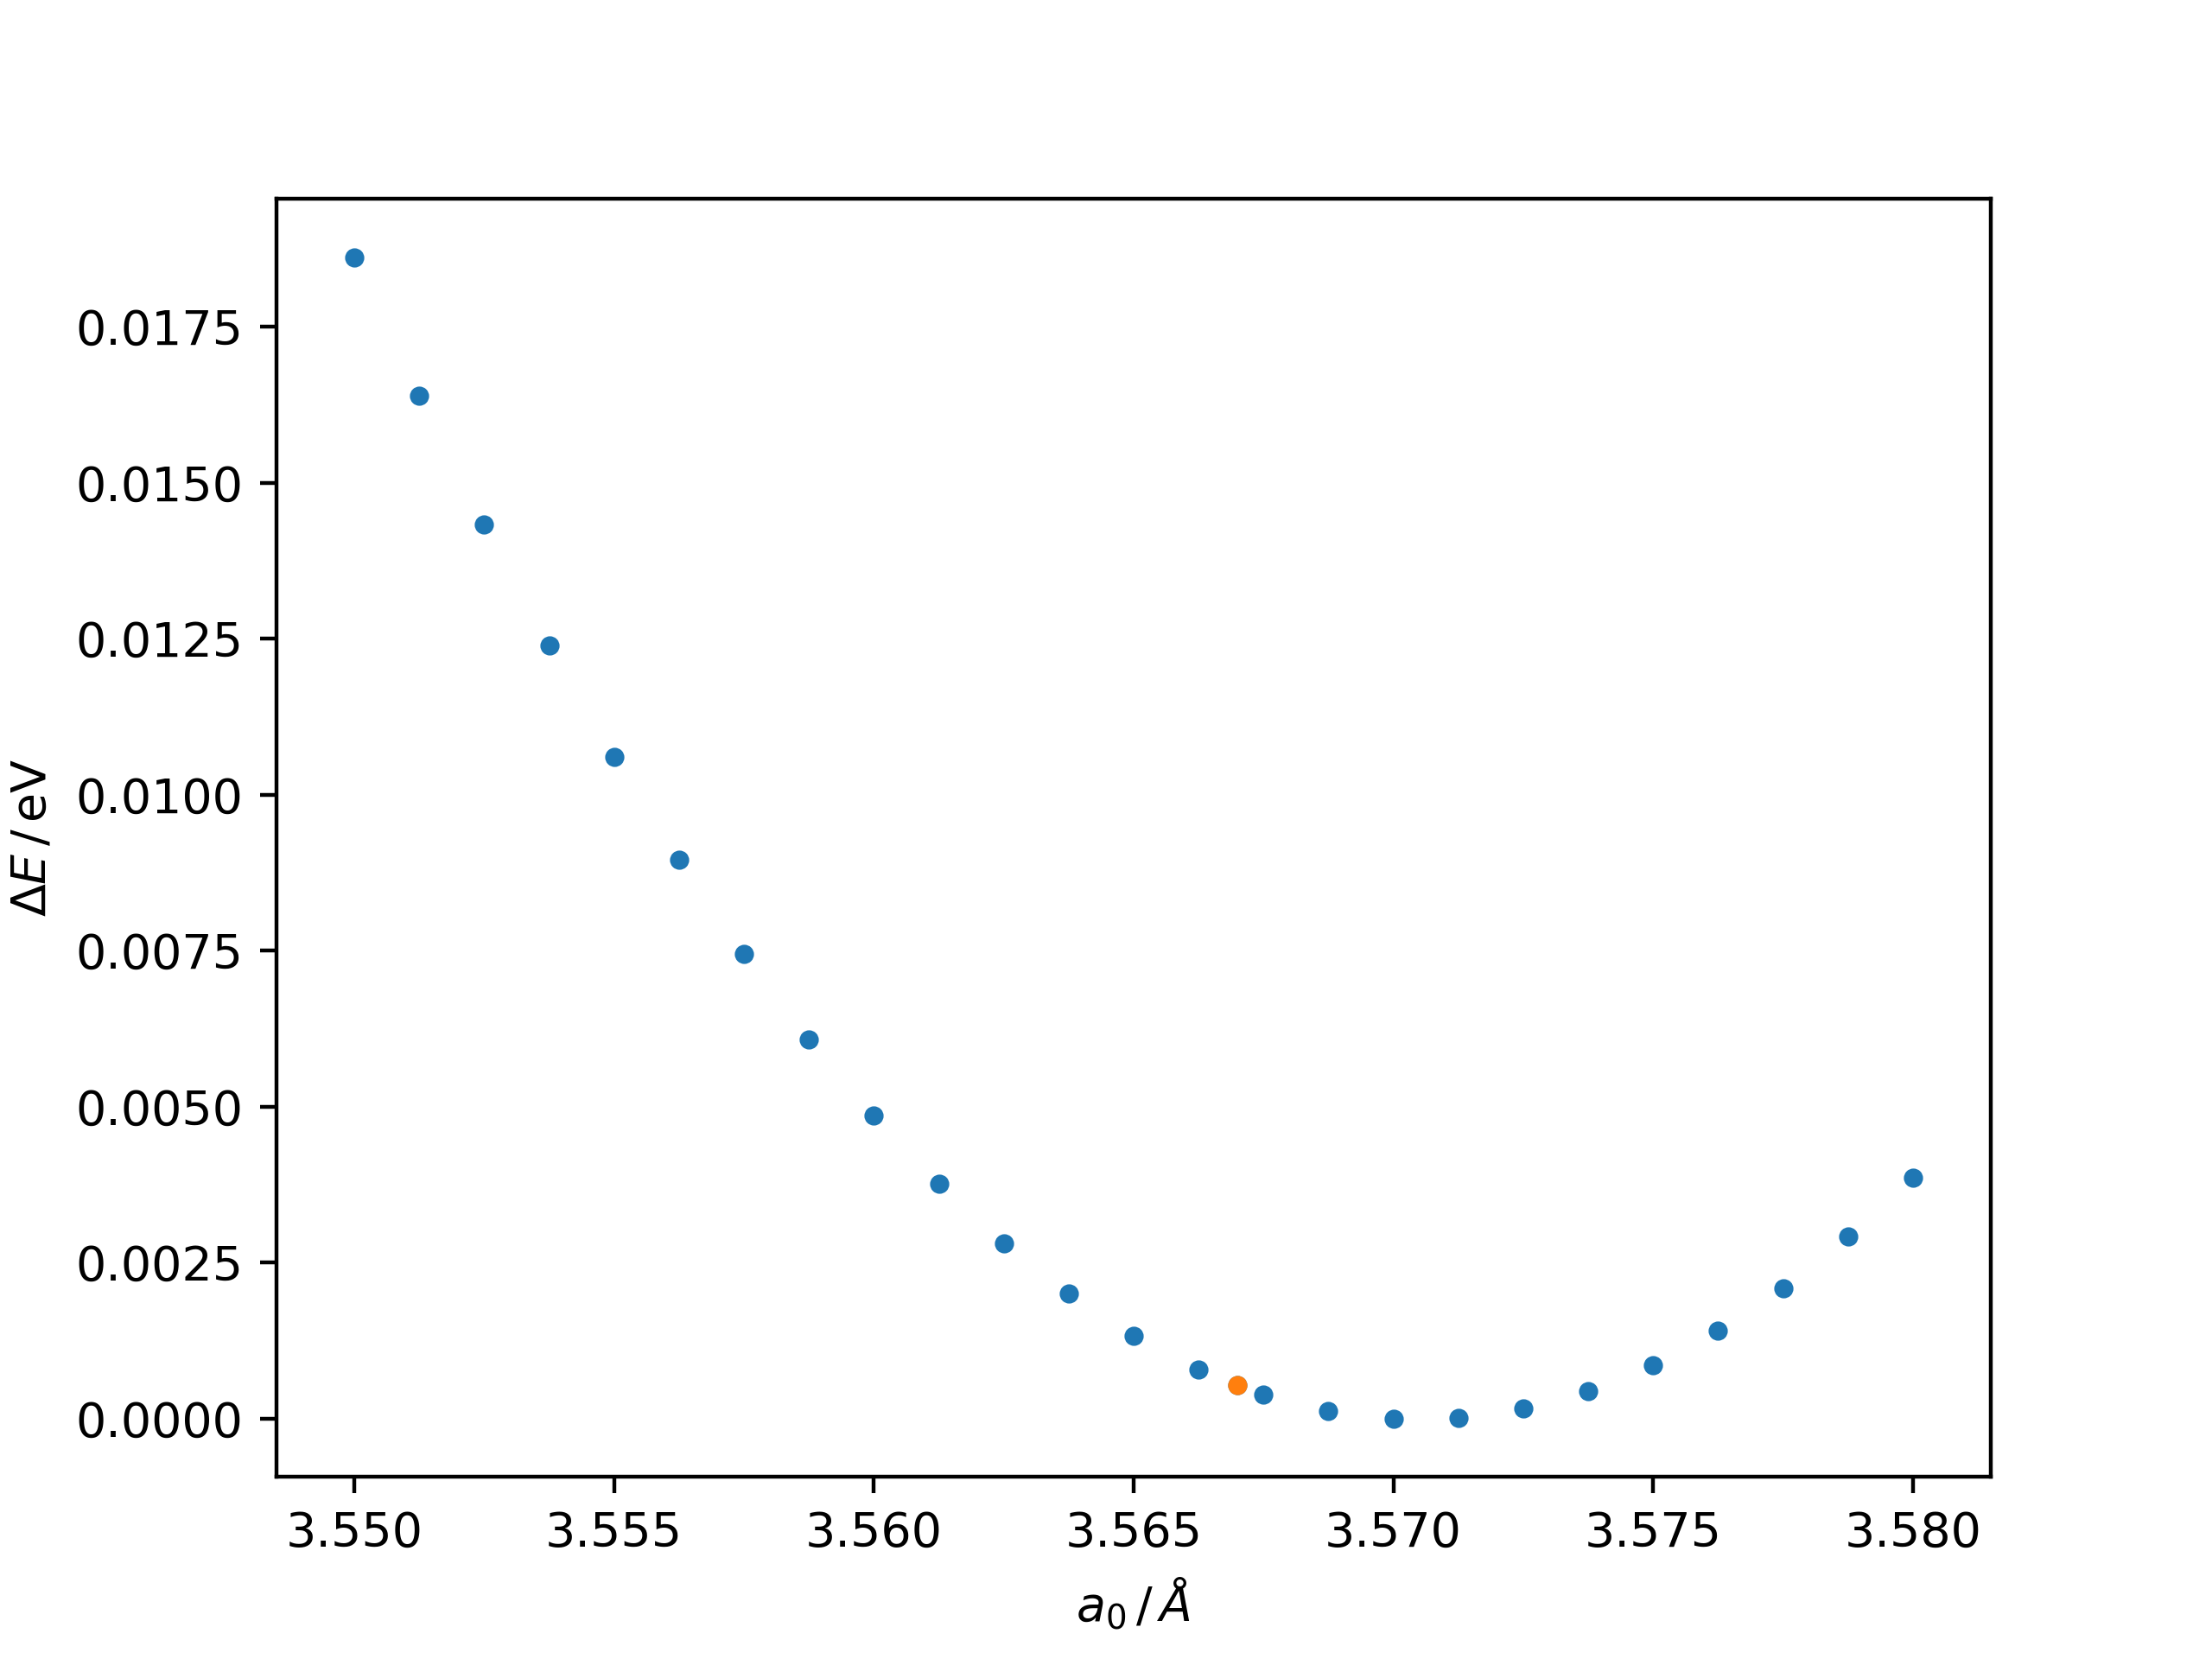
\includegraphics[width=0.55\textwidth]{conv_2.png}
		\resizebox{\columnwidth}{!}{%
		% This file was created with tikzplotlib v0.10.1.
\begin{tikzpicture}

    \definecolor{darkorange25512714}{RGB}{255,127,14}
    \definecolor{darkslategray38}{RGB}{38,38,38}
    \definecolor{lightgray204}{RGB}{204,204,204}
    \definecolor{steelblue31119180}{RGB}{31,119,180}
    
    \begin{axis}[
    axis line style={lightgray204},
    tick align=outside,
    tick pos=left,
    x grid style={lightgray204},
    xlabel=\textcolor{darkslategray38}{\(\displaystyle a_0\, /\, $\AA$\)},
    xmajorgrids,
    xmin=3.5485, xmax=3.5815,
    xtick style={color=darkslategray38},
    y grid style={lightgray204},
    ylabel=\textcolor{darkslategray38}{\(\displaystyle \Delta E\, /\, \text{eV}\)},
    ymajorgrids,
    ymin=-0.000955085049997706, ymax=0.0200567860499518,
    ytick style={color=darkslategray38}
    ]
    \addplot [semithick, steelblue31119180, mark=*, mark size=2.5, mark options={solid}, only marks]
    table {%
    3.55 0.0198728230000143
    3.55125 0.0175824609998472
    3.5525 0.0154342839998662
    3.55375 0.0134278709999762
    3.555 0.0115628649998598
    3.55625 0.00983699399989746
    3.5575 0.0082535789999838
    3.55875 0.00680972199984353
    3.56 0.00550630299994737
    3.56125 0.00434230099995148
    3.5625 0.00331733199982409
    3.56375 0.00243099399995117
    3.565 0.00168264599983559
    3.56625 0.00107228499996381
    3.5675 0.000598451999849203
    3.56875 0.000262742999893817
    3.57 6.28299999334558e-05
    3.57125 0
    3.5725 7.33099998342368e-05
    3.57375 0.000280956999858972
    3.575 0.000624836999804756
    3.57625 0.00110176799989858
    3.5775 0.00171484999987115
    3.57875 0.00246038099999168
    3.58 0.00334101799990094
    3.567 0.000770935999980793
    };
    \addplot [semithick, darkorange25512714, mark=*, mark size=2.5, mark options={solid}, only marks]
    table {%
    3.567 0.000770935999980793
    };
\end{axis}
    
\end{tikzpicture}
    
		}
	\caption{A plot detailing differences in energy of the lowest found lattice constant, the experimentally found value was tested explicitly and can be seen in orange.}
	\label{fig:conv}
\end{figure}

\section{Reorientation of Hydrogen in N$_2$VH}
\label{n2vh}
\subsection{Calculation}
\label{n2vh_calc}
The {\ntvh} defect consists of a vacancy (V) surrounded by two substitutional Nitrogens (N$_2$), with a Hydrogen bonded to one of the two remaining carbon atoms (H). C$_{2v}$ symmetry is reported from EPR runs in both the X ($8-12$\,GHz) and Q-band ($30-50$\,GHz) range \cite{Hartland}. It is not energetically favourable for the Hydrogen to be sit statically in the middle with C$_{2v}$ symmetry; this would suggest that the Hydrogen atom is reorientating between the Carbon atoms fast enough that its position is appearing as an averaged position of the two equivalent sites, giving rise to a higher order of symmetry \cite{Shaw_QT_VH}. 
It has previously been shown for NVH$^-$ that a tunnelling period of $\tau \approx 10^{-8}$, or a tunnelling requency of $0.1$\,GHz, is required to shown an averaged symmetry in EPR \cite{Edwards_N2VH_rate}. It would therefore be of interest to calculate the energy required for this reorientation to occur, and thus potentially create a relationship between tunnelling frequency and temperature. 


A nudged elastic band (NEB) calculation was performed in order to find the energy barrier of the tunnelling path \cite{NEB}.
This method finds a minimum energy path (MEP) between two different states, in this case the Hydrogen moving between two equivalent carbons.
Firstly, a fully relaxed configuration of the two different states are required before any path optimisation can occur.
A diamond lattice was set up with $64$ atoms, one Carbon atom was removed, and two neighbours in the same plane were replaced with Nitrogen atoms, a Hydrogen atom was then placed near one of the two remaining carbon atoms. A geometry optimisation was then carried out in CASTEP in order to find the minimum energy configuration. The PBE functional was used \cite{PBE}, as well as a plane wave cut off energy of $1\,000$\,eV, and an equally spaced Monkhurst-Pack grid of $(4 4 4)$. These values were chosen after a convergence study was performed, with the energy converging to 3 significant figures with these parameters. A finite size effects study should be conducted in the future, however $64$ is a resonably sized unit cell for the accuracy required, as it is theorised that all the electrons surrounding the vacancy point towards it, limiting the negative effects of a small cell size \cite{NVCage}. The system was optimised until no force was over $0.05$\,eV\,\AA$^{-1}$. This was then repeated for the other equivalent Carbon atom. Their energies are within $0.001$\,eV, showing equivalent sites. A C-H bond length of $1.08$\,{\AA} was found, this is consistent with results found in the literature of $1 \pm 0.1$\,{\AA} \cite{N2VH_CH_Bond}.

An initial 'guess' for the unoptimised path between the two systems is needed, for this, a simple a linear trajectory of the Hydrogen atom between the two Carbon atoms along the ($110$) plane was devised. The trajectory contains 7 images, an odd number is used to ensure that it captures the saddle point of the path that is, due to the symmetry of the system, likely to be in the middle of the trajectory. 

The final, optimised, NEB path of the Hydrogen between the two equivalent carbon atoms, is seen in figure \ref{fig:n2vh}. It is of interest that the Hydrogen does not take the shortest straight linear path between each Carbon atom, but instead takes a longer curved path away from the two Nitrogen atoms, possibly avoiding excess electron density. The maximum energy found at the saddle point is $0.536$\,eV, with a full reaction path length of $1.1$\,{\AA}, and a full width half maximum (FWHM) of $0.3781$\,{\AA}, a plot of how energy changes along the reaction coordinate can be seen in figure \ref{fig:n2vh_energy}. This differs from values found in literature, where the reported height and reaction path length are said to be $0.9$\,eV and $0.6$\,{\AA} respectively \cite{Peaker}. There are many differences between these two calculations, namely that \textcite{Peaker} uses a Gaussian basis set, whereas CASTEP uses a plane wave basis set, and the simulation cell is made up of $1\,000$ atoms, the increased number of atoms has the advantage of minimising finite size effects. 

\begin{figure}
	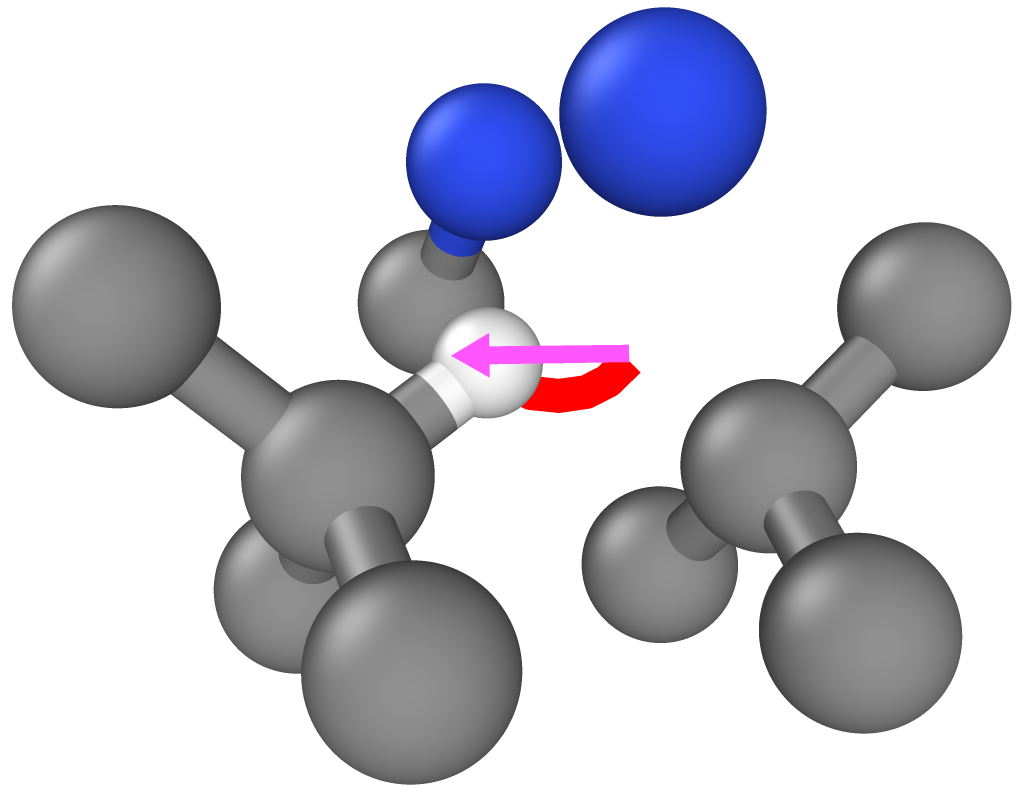
\includegraphics[width=0.4\textwidth]{n2vh_2.png}
	\caption{The NEB path of Hydrogen in \ntvh, where Nitrogen is blue, Carbon is grey, and Hydrogen is white. The \emph{path} is shown in red, and is clearly curved, whilst the raw displacment is shown as a pink arrow. Generated using OVITO \cite{OVITO}.}
	\label{fig:n2vh}
\end{figure}

% \begin{figure}
% 	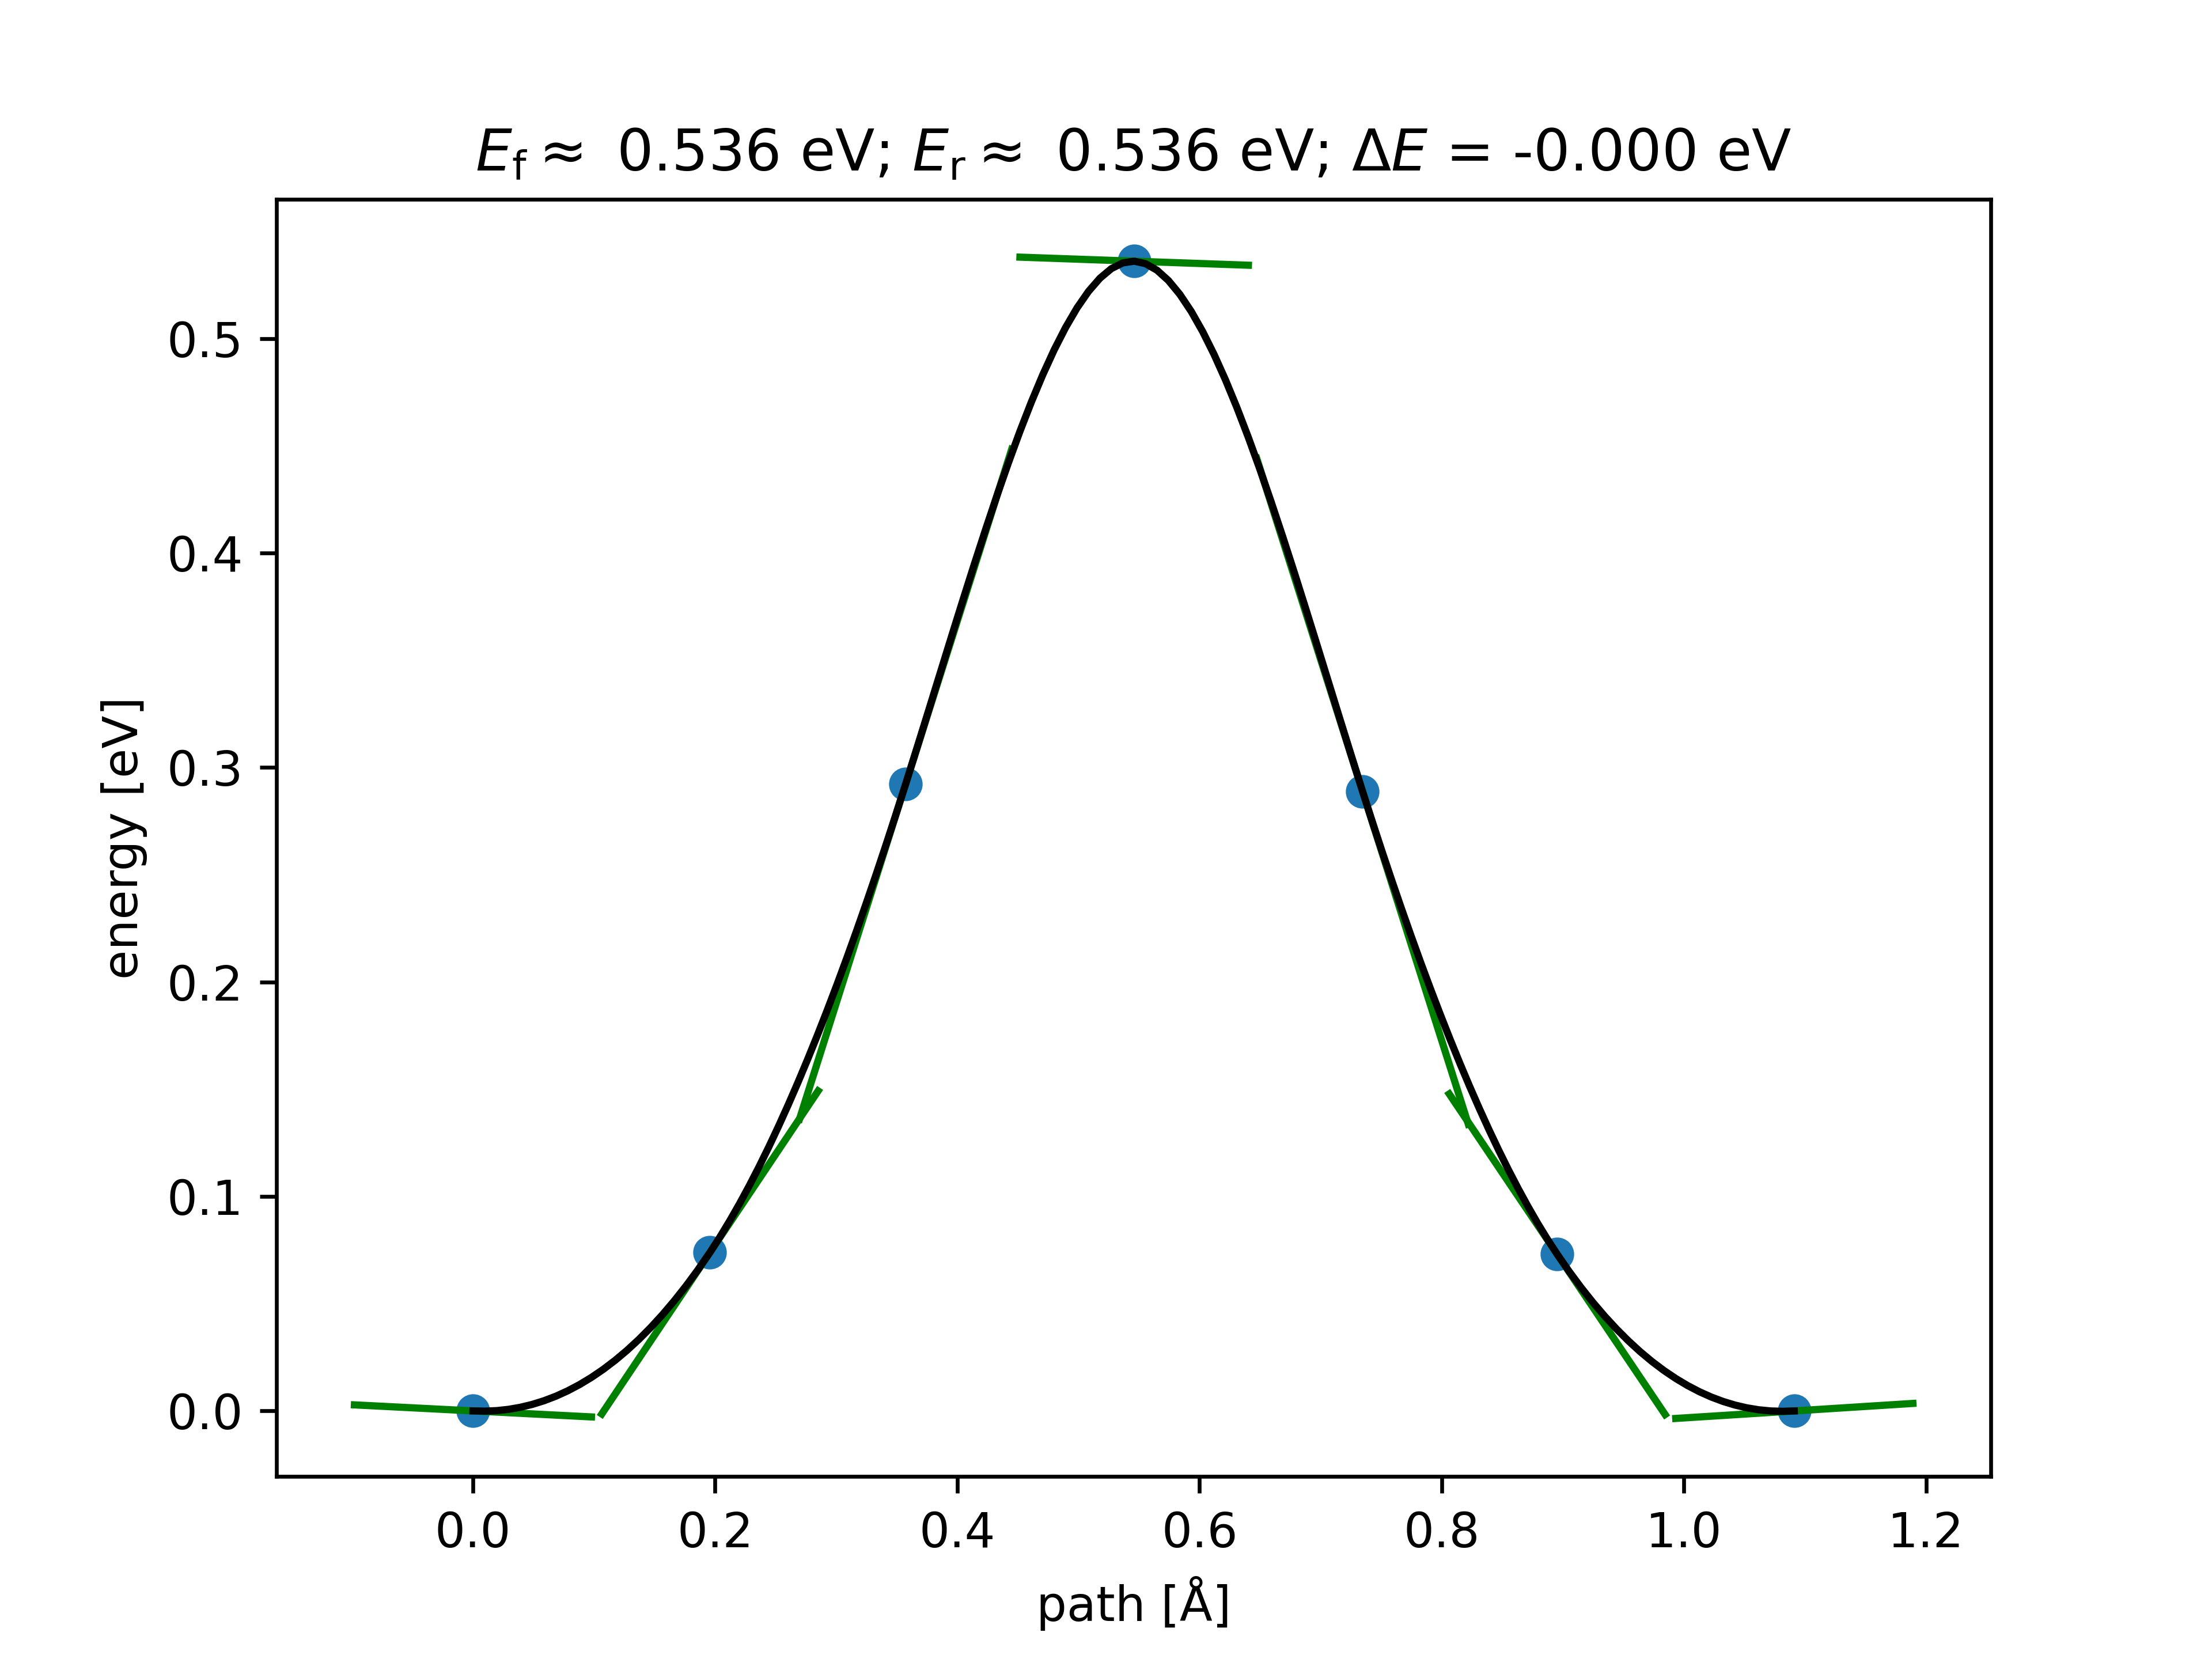
\includegraphics[width=0.56\textwidth]{fig.png}
% 	\caption{The energy along the minimum energy reaction coordinate determined by nudged elastic band calculations. The splines show the gradient of the energy. There is a peak of $0.536$\,eV in the middle.}
% 	\label{fig:n2vh_energy}
% \end{figure}

\begin{figure}
		\resizebox{\columnwidth}{!}{%
		% This file was created with tikzplotlib v0.10.1.
\begin{tikzpicture}

\definecolor{darkslategray38}{RGB}{38,38,38}
\definecolor{green01270}{RGB}{0,127,0}
\definecolor{lightgray204}{RGB}{204,204,204}
\definecolor{steelblue31119180}{RGB}{31,119,180}

\begin{axis}[
axis line style={lightgray204},
tick align=outside,
tick pos=left,
title={\(\displaystyle E_\mathrm{f} \approx\) 0.536 eV; \(\displaystyle E_\mathrm{r} \approx\) 0.536 eV; \(\displaystyle \Delta E\) = 0.000 eV},
x grid style={lightgray204},
xlabel=\textcolor{darkslategray38}{path [Å]},
xmajorgrids,
xmin=-0.162212967524309, xmax=1.25345671309607,
xtick style={color=darkslategray38},
y grid style={lightgray204},
ylabel=\textcolor{darkslategray38}{energy [eV]},
ymajorgrids,
ymin=-0.0305943542901648, ymax=0.565044371318417,
ytick style={color=darkslategray38}
]
\addplot [semithick, steelblue31119180, mark=*, mark size=3, mark options={solid}, only marks]
table {%
0 0
0.195728691355857 0.0738889399999607
0.357308578450571 0.292238490001182
0.546051489841502 0.536086680000153
0.734639424974367 0.288887080001587
0.895362493151131 0.073051770001257
1.0911928918835 -1.95199991139816e-05
};
\addplot [semithick, green01270]
table {%
-0.0978643456779283 0.00280863052526587
0 0
0.0978643456779283 -0.00280863052526587
};
\addplot [semithick, green01270]
table {%
0.106401546743214 -0.00142721633976005
0.195728691355857 0.0738889399999607
0.285055835968499 0.149205096339681
};
\addplot [semithick, green01270]
table {%
0.26972787882916 0.136113977469406
0.357308578450571 0.292238490001182
0.444889278071983 0.448363002532959
};
\addplot [semithick, green01270]
table {%
0.451718778210553 0.537969883790754
0.546051489841502 0.536086680000153
0.64038420147245 0.534203476209552
};
\addplot [semithick, green01270]
table {%
0.647311674146959 0.444067923584384
0.734639424974367 0.288887080001587
0.821967175801774 0.133706236418789
};
\addplot [semithick, green01270]
table {%
0.806224126423847 0.147784812451969
0.895362493151131 0.073051770001257
0.984500859878415 -0.00168127244945537
};
\addplot [semithick, green01270]
table {%
0.993277692517316 -0.00351986676250202
1.0911928918835 -1.95199991139816e-05
1.18910809124969 0.00348082676427406
};
\addplot [semithick, black]
table {%
0 0
0.00978643456779283 -0.000109726991000686
0.0195728691355857 0.000128634865492605
0.0293593037033785 0.000723810656143135
0.0391457382711713 0.00168452546761417
0.0489321728389642 0.00301950438656896
0.058718607406757 0.00473747249967078
0.0685050419745498 0.00684715489358289
0.0782914765423426 0.00935727665496855
0.0880779111101355 0.012276562870491
0.0978643456779283 0.0156137386268136
0.107650780245721 0.0193775290105994
0.117437214813514 0.0235766591085119
0.127223649381307 0.0282198540072143
0.1370100839491 0.0333158387933697
0.146796518516892 0.0388733385536416
0.156582953084685 0.0449010783746931
0.166369387652478 0.0514077833431874
0.176155822220271 0.058402178545788
0.185942256788064 0.065892989069158
0.195728691355857 0.0738889399999607
0.203807685710592 0.0809355347727687
0.211886680065328 0.088445503082435
0.219965674420064 0.0964095262294349
0.2280446687748 0.104818285514244
0.236123663129535 0.113662462237338
0.244202657484271 0.122932737699191
0.252281651839007 0.13261979320028
0.260360646193742 0.14271431004108
0.268439640548478 0.153206969522066
0.276518634903214 0.164088452943714
0.28459762925795 0.175349441606499
0.292676623612685 0.186980616810897
0.300755617967421 0.198972659857382
0.308834612322157 0.211316252046431
0.316913606676893 0.224002074678519
0.324992601031628 0.237020809054121
0.333071595386364 0.250363136473713
0.3411505897411 0.264019738237771
0.349229584095836 0.277981295646768
0.357308578450571 0.292238490001182
0.366745724020118 0.309198092081583
0.376182869589664 0.32635340428984
0.385620015159211 0.343588173313759
0.395057160728757 0.360786145841144
0.404494306298304 0.377831068559802
0.41393145186785 0.394606688157537
0.423368597437397 0.410996751322157
0.432805743006943 0.426885004741466
0.44224288857649 0.442155195103269
0.451680034146036 0.456691069095374
0.461117179715583 0.470376373405583
0.470554325285129 0.483094854721705
0.479991470854676 0.494730259731543
0.489428616424222 0.505166335122904
0.498865761993769 0.514286827583593
0.508302907563315 0.521975483801416
0.517740053132862 0.528116050464178
0.527177198702409 0.532592274259684
0.536614344271955 0.535287901875742
0.546051489841502 0.536086680000151
0.555480886598145 0.534920502448315
0.564910283354788 0.531876213262478
0.574339680111431 0.527070448549225
0.583769076868075 0.520619844415126
0.593198473624718 0.512641036966762
0.602627870381361 0.503250662310707
0.612057267138004 0.492565356553542
0.621486663894648 0.480701755801838
0.630916060651291 0.467776496162179
0.640345457407934 0.453906213741134
0.649774854164577 0.439207544645284
0.659204250921221 0.423797124981206
0.668633647677864 0.407791590855476
0.678063044434507 0.391307578374672
0.68749244119115 0.374461723645371
0.696921837947794 0.357370662774149
0.706351234704437 0.340151031867581
0.71578063146108 0.322919467032248
0.725210028217724 0.305792604374723
0.734639424974367 0.288887080001587
0.742675578383205 0.274754429911811
0.750711731792043 0.260922522804698
0.758747885200881 0.247399846860151
0.76678403860972 0.234194890258074
0.774820192018558 0.221316141178368
0.782856345427396 0.208772087800936
0.790892498836234 0.196571218305681
0.798928652245072 0.184722020872507
0.806964805653911 0.173232983681315
0.815000959062749 0.162112594912009
0.823037112471587 0.151369342744491
0.831073265880425 0.141011715358664
0.839109419289264 0.131048200934431
0.847145572698102 0.121487287651694
0.85518172610694 0.112337463690357
0.863217879515778 0.103607217230322
0.871254032924616 0.0953050364514918
0.879290186333455 0.0874394095337692
0.887326339742293 0.0800188246570566
0.895362493151131 0.0730517700012578
0.90515401308775 0.0650966201264929
0.914945533024368 0.0576439473317834
0.924737052960987 0.0506854718472018
0.934528572897605 0.044212913902824
0.944320092834224 0.0382179937287228
0.954111612770842 0.0326924315549735
0.963903132707461 0.0276279476116503
0.973694652644079 0.0230162621288259
0.983486172580698 0.0188490953365759
0.993277692517316 0.0151181674649732
1.00306921245393 0.0118151987440926
1.01286073239055 0.00893190940400856
1.02265225232717 0.00646001967479481
1.03244377226379 0.00439124978652394
1.04223529220041 0.00271731996927294
1.05202681213703 0.00142995045311345
1.06181833207365 0.000520861468122469
1.07160985201026 -1.82267556292359e-05
1.08140137194688 -0.00019559398806468
1.0911928918835 -1.95199991139816e-05
};
\end{axis}

\end{tikzpicture}

		}
		\caption{The energy along the minimum energy reaction coordinate determined by nudged elastic band calculations. The green splines show the gradient of the energy, which is used for interpolation. There is a peak of $0.536$\,eV in the middle.}
		\label{fig:n2vh_energy}
\end{figure}



\textcite{Peaker} takes the width of the barrier as the \emph{displacement} of the Hydrogen atom, the difference between the initial and final configuration. A higher displacement of $0.89$\,{\AA} was found here, however taking the raw displacement of the Hydrogen atom does not account for the path it takes during reorientation, nor does it fully utilise the minimum energy path that the NEB calculation found. A more appropriate approximation would be to take the fully optimised path of the Hydrogen atom as the width of the barrier, and so to map the potential energy barrier to the Hydrogen path, instead of the reaction coordinate. This is reasonable as the majority of the movement stems from the Hydrogen, with the carbon atoms slightly relaxing under bond breaking and forming. The full path of the Hydrogen atom is $1$\,{\AA}, only $0.1$\,{\AA} less than the full reaction coordinate. The potential barrier height was found to be almost half of that found in the literature, this could be due to a more optimised MEP, or a more accurate basis. The \emph{first} unoptimised MEP has a barrier height of $0.844$\,eV, much closer to that found in the literature. 
\subsection{Analysis}
With a barrier height and width determined it is now possible to calculate the probabilities of overcoming the barrier. As the barrier is a non-trivial shape, two different approximations will be made for different uses: approximating the barrier as a finite square potential, and the WKB potential. 

For the finite square potential, it is common to take the FWHM as the width, and the saddle point as the barrier height. The classical rate of reoritentation can be calculated as 
\begin{align}
    \label{classical}
    \Gamma &= A\exp({\frac{-E_a}{k_BT}})
\end{align}
where $A$ is the attempt frequency, $E_a$ is the activation energy, taken to be the barrier height, $k_B$ is Boltzmann's constant, and $T$ is the temperature \cite{Peaker}. The frequency in the direction of the barrier was found to be $40.87$\,THz. This would give a classical reorientation rate of $\Gamma = 0.0405$\,GHz at room temperature, at $10$\,K this is approximately zero. At room temperature this is still quite fast, but an order of magnitude lower than would be required to see an averaged symmetry in EPR. As EPR is performed at temperatures at or below $10$\,K it is likely that the Hydrogen is quantum tunnelling. 

Taking the finite square potential approximation, the probability the Hydrogen atom tunnelling can be calculated as 
\begin{align}
    \label{square}
    P &= \exp(\frac{-4a\pi}{h}\sqrt{2m(V-E)})
\end{align}

where $a$ is the width of the barrier, taken to be the FWHM, $m$ is the mass of the tunnelling particle, $V$ is the potential energy of the barrier, and $E$ is the energy of the particle. As an approximation the ground state energy of the Hydrogen atom can be taken as that of a simple harmonic oscillator 
\begin{align}
    E_0 = \frac{1}{2}h\nu
\end{align}
where $\nu$ is the frequency of the oscillations. The frequency of the hydrogen atom was $40.87$\,THz (section \ref{phonon}), such that the ground state energy was thus $0.0845$\,eV. As EPR is typically performed at temperatures below $10$\,K, it is sensible to assume that the Hydrogen is in its ground state. This energy value can then be used in in equation \ref{square} to give a probability of tunnelling to be $P = 1.4\cross10^{-5}$. The tunnelling rate can then be calculated similarly to \ref{classical} as shown below, where $A$ is the attempt frequency. 
\begin{align}
    \Gamma &= A\cdot P
\end{align}
Giving a final tunnelling rate of $0.59$\,GHz for the square potential barrier. This is in the range of frequency for which an averaged C$_{2v}$ symmetry would be measured by EPR, giving a similar result to other N$_{n}$VH defects.


A more accurate approximation of the nature of the potential barrier is the WKB approximation. This takes the form of 
\begin{align}
    P &= \exp(\frac{-4\pi}{h}\int_{a}^{b}\sqrt{2m(V(x)-E)}{\d}x)
\end{align}
where $a$ and $b$ are the \emph{turning points} of the barrier, such that $V(x) = E$ \cite{butorac}. This approximation retains the shape of the barrier. This results in a rate of $\Gamma = 0.126$\,GHz, once again, this is within the range to give an averaged symmetry. 


\subsection{Phonon Calculations}
\label{phonon}
In order to calculate the tunnelling rate, the attempt frequency must first be calculated. Just using the stretch mode as the attempt frequency can be a good approximation, however as the Hydrogen takes a very particular path the direction of the vibration becoomes quite important, so it must be factored into the calculation.
This can be done through a finite displacement phonon calculation, allowing the calculation of the frequency at which the Hydrogen atom vibrates in the direction of the minimum energy path. This calcualtion uses the optimised system found in section \ref{n2vh_calc}. To find the frequencies and magnitudes at which the atoms vibrate, a finite-displacement phonon calculation was performed in CASTEP \cite{DynamicalMatrix}. In this, each atom is separately moved a small displacement from its origin (in this case $0.02$\,{\AA}), and the forces acting upon the atom calculated. This results in a $3N\times3N$ \emph{dynamical matrix} that contains the force created on each atom due to the displacement of an atom from the origin \emph{i.e.} the force constants. More mathematically this is the second derivative of energy with respect to the atomic displacements, shown in equation \ref{eqn:dynmat}. Where $r_n$ is the position of an atom, and $m_n$ is its corresponding mass.

\begin{equation}
	\label{eqn:dynmat}
	\frac{\d^2E}{ {\d}r_i {\d}r_j} \frac{1}{\sqrt{m_i m_j}}
\end{equation}



This dynamical matrix can then be diagonalised, to retrieve its eigenvectors and eigenvalues. The eigenvalues are the square of the wavenumbers, and the eigenvectors detail the strength of a mode and its direction. To calculate the frequency at which the Hydrogen vibrates in the direction of the MEP, the dot product between the eigenvectors, $\hat{e}$, and the \emph{normalised} direction of the MEP, $\hat{r}_H$, is multiplied by the corresponding wavenumber of each eigenvector, as shown below. 
\begin{align}
    \nu_{\text{MEP}} = \sum_{i}^{3N} \nu_i (\hat{e_i} \cdot \hat{r}_H) &\approx 40.872\,\text{THz}\\ 
	&= 1363\,\text{cm}^{-1} \nonumber
\end{align}
This is of the correct order of magnitude for a H-C bond vibration, and is also close to the theorised transition mode between $1375$ and $1378$ cm$^{-1}$ \cite{Peaker,Hartland}.

\subsection{Further Calculations}
The tunnelling rates, whilst lower than the rate of EPR, are not lower than required for an averaged frequency to be shown \cite{Hartland}. This is in agreement with experiment, however it is possible that the rates are still underestimated, or even overestimated. Another run of the NEB path should be undertaken with a larger cell, and potentially a more accurate meta-GGA functional, such as HSE06 \cite{HSE06}. 

The MEP is only a line in space, and as such all of the calculations for tunnelling are in that single direction in space.
There is the possibility of there being an area around the MEP that has an energy very close to that of the MEP, such that it is possible for the Hydrogen atom to tunnell across a variety of different paths surrounding the MEP, this would greatly increase the tunnelling probability. To capture this behaviour, a path integral molecular dynamics (PIMD) simulation will have to be run. PIMD uses the Feynman path-integral formulation of quantum mechanics,  which represents the quantum mechanical propogator as a sum over all possible paths that the particle can take, in order to approximate the quantum behaviour of the non-electronic (\emph{i.e. nucleic}) part of the system. This would allow for a much more accurate calculation, fully taking into account all quantum mechanical effects. 
Before this can be done however, a suitable potential will have to first be identified. A suitable candidate is the MACE-MP-0 \cite{MACE} potential, mentioned in section \ref{sec:future}, further investigations will have to undertaken, and extra training of the potential may be required before it is suitable to run a full PIMD calculation.

%Put this bit in later 
%This path is the reaction coordinate, so it accounts for the movement of every atom, however the majority of the movement stems from the Hydrogen, with the carbon atoms slightly relaxing under bond breaking and forming. This makes it possible to map the energy from the reaction coordinate, which has a length of $1.1$\,\AA to the Hydrogen atom's path, which has a length of $1$\,\AA. The small difference between these two values makes it a reasonable approximation to make.



\section{Vacancy Migration in a Diamond ($001$) Surface}
\label{sec:vacancy}
There is much concern of how to remove vacancies from diamond, in order to create a perfect crystal. Annealing techniques are used to heat the diamond up to a certain temperature and cool it down, in hopes of making the vacancies turn mobile and rising to the surface, effectively eliminating themselves from the bulk. Previous experimental results have shown that this starts to occur at ~$700$\,K, however it could also be useful to know the energies required for a vacancy to migrate, and also the energy barrier involved for the formation of a vacancy \cite{VacancyTemp}. Molecular dynamics simulations can provide an insight into the mechanisms involved in vacancy migration, and to inform later experiments. Hu \al, as shown in section \ref{Hu}, have used a tersoff potential to model the vacancy migration of an atom from the second layer of a diamond ($001$) surface to the top layer \cite{hu}.
%Their results showed that this process begins to occur at $1400$\,K, deviating from known experimental results. Hu {\al} argue that is due to how the temperature of the diamond is measured in experiments, that the temperature of the surface is in fact much higher than that of the substrate which is being measured, and so would align more with their findings. 
The results of Hu {\al} are quite old, however the methods used are not out of date, so it is reasonable to try and recreate similar results, and expand upon their work using more state-of-the-art techniques. 
\subsection{Molecular Dynamics}
The same system was set up as Hu {\al} described in section \ref{Hu}: a $1$\,fs timestep was used, as well as a $100$\,fs timestep for the velocity rescaling method, and a $1\,000$\,fs timestep for the pressure rescaling method. There is no mention in the original paper what the timestep for the velocity rescaling method is, nor is a pressure rescaling method used at all. The Berendsen barostat was used to ensure that the crystal can expand slightly under higher temperatures to avoid excess strain on the crystal. The Tersoff many-body potential was used \cite{Tersoff}. Following Hu {\al}, an initial system was created and relaxed at $300$\,K for $5$\,ps, before a vacancy was created in the second layer and it was allowed to relax again for another $5$\,ps. The final configuration of this system formed the starting configuration of all further simulations. The system was then allowed to run at temperatures in the $300$ -- $2\,000$\,K range. Taking inspiration from Hu {\al}, the positions of the atoms neighbouring the vacancy were extracted from the MD run. The atom with the lowest average distance to the vacancy site was taken to be the atom that was moving into the vacancy to switch places with it, which was then used for analysis. 
\subsection{Analysis}
The diffusion coefficient can be found as 
\begin{align}
	D = \frac{\langle u^2 \rangle}{2N_dt}
\end{align}
where $\langle u^2 \rangle$ is the mean squared displacement of the atom, $N_d$ is the dimentionality (\emph{e.g.} 3), and $t$ is the time over which the mean squared displacement is taken. The diffusion coefficient can be determined by taking the slope of the mean squared displacement. The diffusion barrier, $E_m$, can then be calculated by using the Arrhenius equation, shown in equation \ref{eqn:arr}, where $D_0$ is a prefactor. 
\begin{align}
	\label{eqn:arr}
	D = D_0 \exp(\frac{E_m}{k_BT})
\end{align}

A plot of $\ln(D)$ against $\frac{1}{k_BT}$ can be seen in figure \ref{fig:arr}, taking the slope of this plot gives the diffusion barrier $E_m = 0.25$\,eV, whilst taking the exponential of the intercept gives the prefactor $D_0 = 1.92\times10^{-6}$\,cm$^2$s$^{-1}$. This is not too close to the results of Hu \al, which found $E_m = 0.42$\,eV and $D_0 = 3.69\times10^{-6}$\,cm$^2$s$^{-1}$ \cite{hu}. One reason for this difference between results is the seemingly \emph{ad hoc} decisions made when dealing with dealing with calcualting the diffusion coeffcients, a more rigorous approach should be used in the future, to hopefully keep any future results obtained consistent \cite{DiffusionRigorous}. 

Despite differences in calculated constants, similar behaviour is seen in terms of temperature at which diffusion occurs. With temperatures below $1\,000$\,K not diffussing at all, those between $1\,000$ and $1\,300$\,K diffussing to an intermediate position, and those in the range of $1\,400$ -- $1\,800$\,K relaxing to an intermediate position, before fully relaxing into the vacancy site. At high temperatures above $2\,000$\,K, diffusion sometimes occurs, and other times the surface neighbours of the vacancy are dislocated, and move away from the vacancy, essentially creating a divacancy on the surface. 

% \begin{figure}
% 	\includegraphics*[width=0.55\textwidth]{hu.png}
% 	\caption{Plot of $\ln(D)$ against $\frac{1}{k_BT}$ derived from  Arrhenius equation, the slope corresponds  to the activation barrier, whilst the intercept is simply a prefactor.}
% 	\label{fig:arr}
% \end{figure}

\begin{figure}
	% 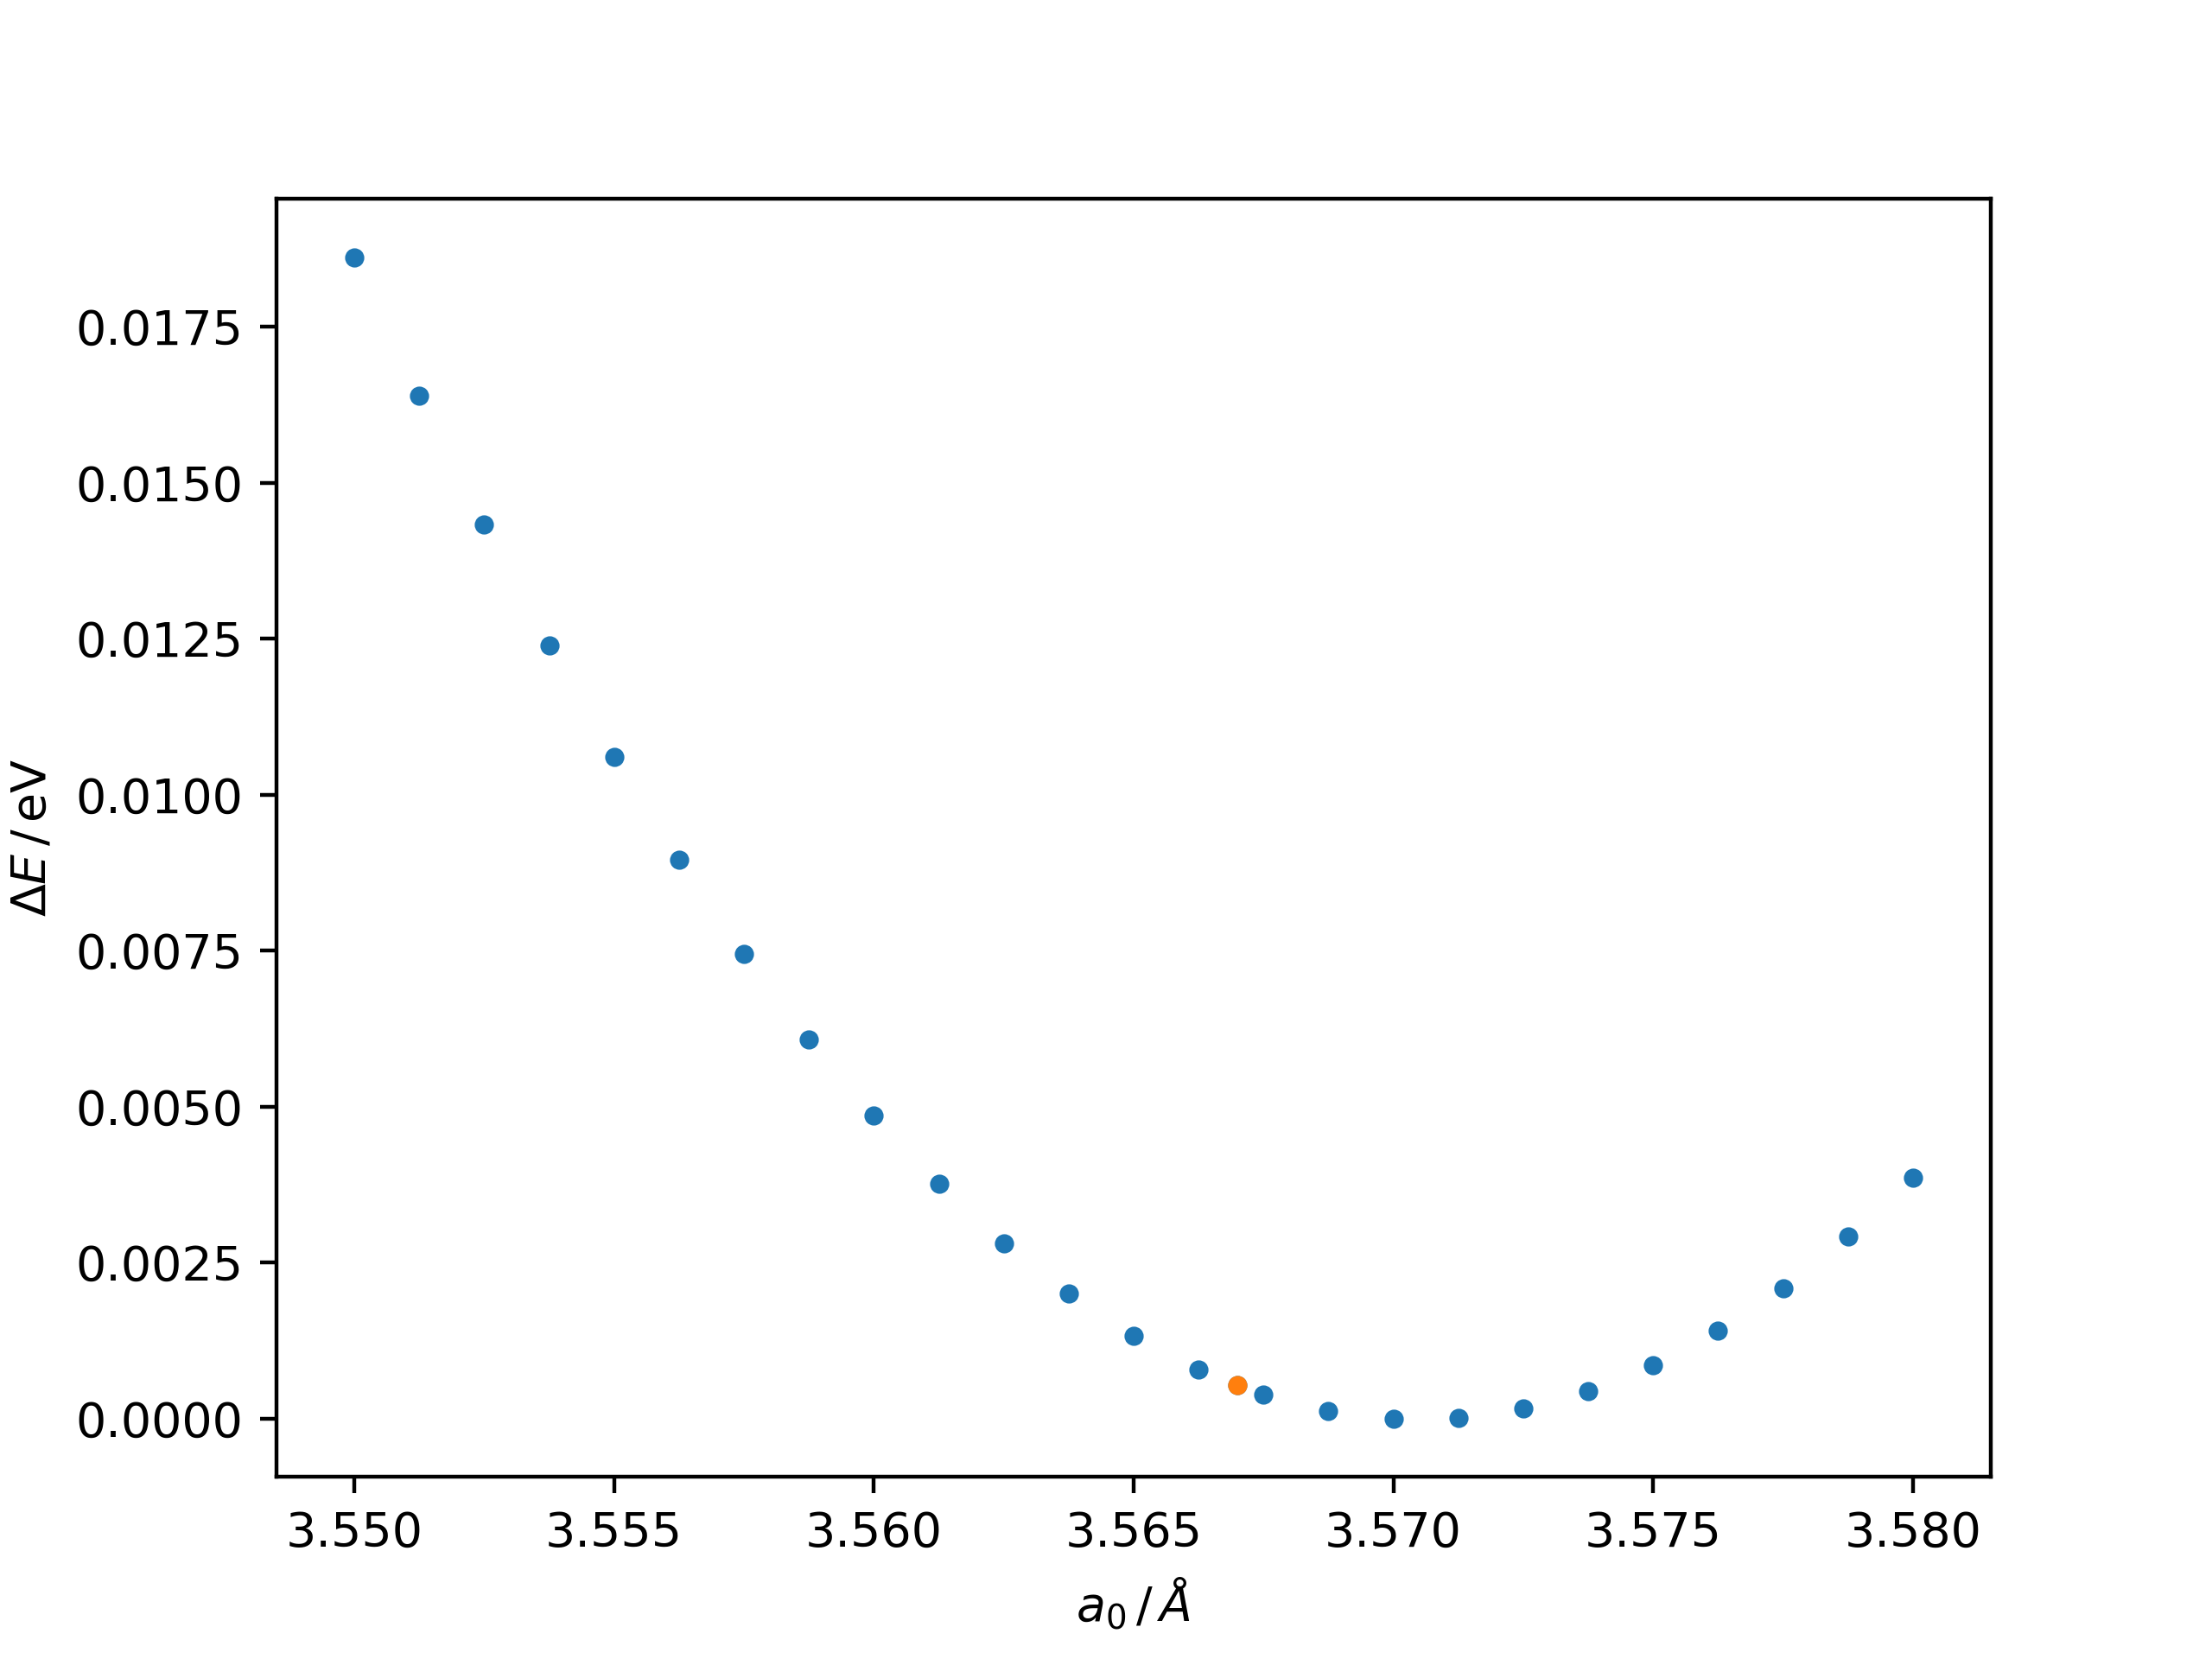
\includegraphics[width=0.55\textwidth]{conv_2.png}
		\resizebox{\columnwidth}{!}{%
		% This file was created with tikzplotlib v0.10.1.
\begin{tikzpicture}

    \definecolor{darkorange25512714}{RGB}{255,127,14}
    \definecolor{darkslategray38}{RGB}{38,38,38}
    \definecolor{lightgray204}{RGB}{204,204,204}
    \definecolor{steelblue31119180}{RGB}{31,119,180}
    
    \begin{axis}[
        axis line style={lightgray204},
        tick align=outside,
        tick pos=left,
        x grid style={lightgray204},
        xlabel=\textcolor{darkslategray38}{$(k_BT)^{-1}$\,/\,eV},
        xmajorgrids,
        xmin=6.04375, xmax=14.9079166666667,
        xtick style={color=darkslategray38},
        y grid style={lightgray204},
        ylabel=\textcolor{darkslategray38}{ln$(D$\,/\,cm$^{2}$s$^{-1})$},
        ymajorgrids,
        ymin=-17.5376466719308, ymax=-15.9459591729106,
        ytick style={color=darkslategray38}
        ]
        \addplot [semithick, steelblue31119180]
        table {%
        14.505 -17.4652972401572
        11.604 -16.9443813313869
        9.67 -16.5971040588734
        8.28857142857143 -16.3490488642209
        7.2525 -16.1630074682316
        6.44666666666667 -16.0183086046843
        };
        \addplot [semithick, darkorange25512714, mark=*, mark size=2.5, mark options={solid}, only marks]
        table {%
        14.505 -17.460244170299
        11.604 -16.8859780999683
        9.67 -16.8081805578708
        8.28857142857143 -16.1609556572895
        7.2525 -16.1729401820324
        6.44666666666667 -16.0488489000943
        };
        \end{axis}
    
    \end{tikzpicture}
    
		}
		\caption{Plot of $\ln(D)$ against $\frac{1}{k_BT}$ derived from  Arrhenius equation, the slope corresponds  to the activation barrier, whilst the intercept is simply a prefactor.}
		\label{fig:arr}
\end{figure}


\subsection{Further Research}
This section has focused entirely on surface migrations in the ($001$) surface, however diamond has many more interesting surfaces. Further molecular dynamics simulations of vacancy migration in different surfaces should be undertaken, such as the ($111$) surface, as well as calculations of vacancy migration from different depths from the surface. Migration in the bulk of diamond should also be investigated.
As mentioned in section \ref{sec:future}, the more accurate MACE-MP-0 potential \cite{MACE} should be used. 

Monte Carlo simulations can also be carried out, using data from DFT to inform the parameters of these simulations, such as the energy barrier of diffusion \cite{radiation_modelling, HybridMonteCarlo}. This can allow to incorporate the accuracy of DFT in molecular dynamics time scales. This requires a large amount of data to be collected, as Monte Carlo simulations do not calculate any parameters of the system, and instead rely on inputed data, therefore data about every possible vacancy configuration is needed. This can quickly grow out of hand if modelling more than three vacancies in close proximity, as cell sizes will need to grow to accomodate this. Nonetheless, the data required for these simulations is still useful on its own.

%Basically 1600 is when it really starts to migrate properly, we see two-step (maybe even three step) migration at 1600 and above, it does happen at 1400 but not always, probably a high chance of randomness -> monte carlo, at 2000 strange things happen because it is so hot, tersoff may be "breaking down". For GAP it seems to migrate at EVERY temperature, not good, we also see no migration from the third at any temperature for gap, also not good, could just be (001) surface however . Maybe explore NVT instead of NPT properly? -> makes no difference THEY USE CM^2 / s -> CHECK UNITS AND CONVERT


\section{Key Text Review}

\subsection{First Principles Study of Point Defects in Diamond}
\textcite{Peaker} carries out computational simulations on a wide variety of point defects in diamond. All calculations were done using DFT implemented in AIMPRO \cite{AIMPRO}, using the PBE exchange-correlation functional \cite{PBE}. AIMPRO uses Gaussian basis sets centred on each atom, as opposed to the plane-wave method used for the original research in this paper. A $1\,000$ atom supercell is used before introducing any defects, leaving some systems with one fewer or one more atoms depending on the defect being studied. Periodic boundary conditions are applied such that they satisfy Bloch's theorem \cite{Bloch}. 

Defects containing Nitrogen, vacancies, and Hydrogen were explored, where $n +m = 0, 1, 2, 3, 4$ in N$_n$VH$_m$, this is clearly incredibly broad, so the entire paper cannot be covered in depth in this short review. The defects are lumped into groups depending on the sum of $n$ and $m$, for each of these groups structural, electrical and vibrtaional properties are calculated, as well as the electronic structure and hyperfine interaction.

A section of the paper is devoted to the quantum tunnelling effects of different defects, including {\ntvh}, with a nudged elastic band calculation being performed, calculating the barrier height and width. Further calculations to find out the rate of quantum tunnelling are not explored by the author, however classical rates of site reoreintation are estimated. The lack of concrete rate calculations was the inspiration for section \ref{n2vh_calc} of this paper.

The binding energies of the defects were also investigated, with stability being correlated with an increased number of Nitrogen and Hydrogen in a defect. From this the energetics of defects combining to form new defects were calculated, including any intermediate stages. 

``First principles study of point defects in diamond'' was of great use to my research due its breadth, and despite its different calculatory methods, it will certainly be useful in the future. 

\subsection{Diffusion of Vacancies Near a Diamond ($001$) Surface}
\label{Hu}
``The Diffusion of Vacancies Near a Diamond ($001$) Surface'' by Hu \al~has played an important role in my research, influencing a large part of section \ref{sec:vacancy}. Hu \al used molecular dynamics to investigate vacancy diffusion in diamond surfaces at various temperatures, calculating the diffusion coefficient and diffusion barrier. Knowing the properties of vacancy defects, and at what temperatures they are mobile such that they might escape to the surface is important when dealing with synthetic diamodns. The paper is limited in that it only deals with vacancies found in the second layer of the ($001$) surface. Other surfaces, such as the cleavage ($111$) surface, also play important roles in experiment, not to mention vacancies that are found further into the bulk, such as in the third or fourth layer.

They construct their simulation as a unit cell repeated equally $5$ times in all $3$ cardinal directions, with periodic boundary conditions along the $x$ and $y$ axes, and the surfaces in the $z$ direction showing a ($001$) face. There is no mention of the boundaries of the cell in the $z$ direction, however as it is dealing with a surface diffusion, it is reasonable to assume that there is a sufficent vacuum gap, such that there are no external forces acting on the surface. The perfect diamond crystal is first allowed to relax for $5$\,ps at $300$\,K, before having an atom in the second layer removed, and then relaxed for another $5$\,ps. The final configuration of this system was then used as the starting point of all subsequent simulations, allowing for consistency between them all. The system is then ran for up to $35$\,ps at temperatures ranging from $300$ -- $2\,000$\,K. 

As it is impossible to precisely track a vacancy in a crytal, as it does not truly exist, Hu {\al} opt instead to measure the displacement of the vacancy's nearest neighbours in the surface, as vacancies move by exchanging positions with one of their neighbours. It is only necessary to measure the positions in the surface, as \textcite{Halicioglu} previously determined that it is energetically unfavourable for a vacancy to diffuse deeper into the bulk. 

Hu \al found that full vacancy migration is only achieved at and above $1\,400$\,K, with simulations ran in the $1000$--$1\,300$\,K range showing only a partial relaxation of the surface neighbours into an intermediate position which they remain in until the end of the simulation. For $1\,400$--$1\,800$\,K, the surface neighbour relaxes to the intermediate position for some time, before finally moving all the way to the vacancy site, implying that the vacancy has fully migrated to the surface. Hu \al~claim that this is the first time that the two-step migration phenomena has been observed, with the intermediate vacancy position being much closer to the neighbour's original site than the vacancy site. For $2\,000$\,K the surface neighbour migrates to the vacancy site fully in one motion. These results differ to those seen in experiment, as mentioned in the paper, \textcite{Davies} have showed that in Type IIa diamond, the vacancy concentration greatly decreases after annealing at a temperature range of $973$--$1\,023$\,K. This would imply that the vacancy is fully mobile, as was seen in the simulations above $1\,400$\,K. This discrepancy is explained by Hu \al~to be caused by how the temperatures are read: Davies \al~are measuring the temeprature of the substrate on which the diamond is grown, however the temperature of the surface is likely to be much hotter. Another cause of the higher required migration temperature observed by Hu \al could be due to the use of the Tersoff potential, which is likely to overbind in cases like these, stopping the vacancy from migrating at the correct temperature.

A final diffusion energy barrier was found, the methodology of which can be seen in section \ref{sec:vacancy}, $E_m = 0.42$\,eV, this is much lower than the rest of the literature would suggest, however diffusion near the surface is expected to have a much lower energy barrier.

\subsection{Nitrogen in Diamond}
``Nitrogen in Diamond'' is a comprehensive literature review of the Nitrogen defect centres in diamond \cite{NitrogeninDiamond}. 
The paper outlines the two main methods of preparing lab-grown diamonds, chemical vapour disposition (CVD) and high pressure high temperature (HPHT). Details are given on how different types of impurities occur during production and how to mitigate or encourage them. As Nitrogen is by far the largest impurity in diamond, the main interest of the paper is the section detailing the properties that different Nitrgoen-based defects have, including many ways they can be identified through different types of spectroscopy. The paper is far too large and varied for a full review, so a focused review of things that relate directly to the research carried out in this paper, and potential candidates for future research, will instead be conducted. 

Of interest are the interstitial Nitrogen defects, N$_i$ and N$_{2i}$, which are simpy a Carbon atom replaced with one or two Nitrogen atoms respectively, in the case of N$_{2i}$, these two Nitrogen atoms are neighbours. EPR spectra have been suggested for the structure, however their signals are not supported by DFT calculations \cite{Atumi_2013}. More research of this elusive defect is required, which could be carried out in the future.

Reorientation of Hydrogen in N$_n$VH defects, where $n$ ranges from $1$ to $3$ was all covered. All of these defects are formed around a central vacancy, with a Hydrogen in the middle of the vacancy, and Nitrogens replacing the surrounding Carbons to varying degrees. In the case of NVH, EPR spectra and hyperfine interactions all report a C$_{3v}$ symmetry, which initially would imply that the Hydrogen is directly bonded to the Nitrogen, and thus sits in the centre towards the vacancy in the ($1 1 1$) plane. However the dangling bond on the Nitrogen would make this an energetically unfavourable position to be in \cite{Goss_NVH}. This problem is rectified by identifying that the Hydrogen is in fact quantum tunnelling between the three carbon sites at rates similar to that of EPR, giving it an averaged C$_{3v}$ symmetry \cite{Shaw_QT_VH}. The time scales do not in fact need to be \emph{faster} than the rate at which EPR is run, it can in fact be an order of magnitude lower, with a frequency of roughly $0.1$\,GHz \cite{Edwards_N2VH_rate}.

The more recently identified N$_{2}$VH defect also undergoes a similar reorientation, appearing as an averaged C$_{2v}$ symmetry instead of a C$_{1h}$ symmetry under EPR \cite{Peaker}. Comprehensive calculations are still needed to determine the rate at which the Hydrogen tunnels, which is the inspriation for section \ref{n2vh}. 

N$_{3}$VH is the final member of the N$_{n}$VH family, as every bond pointing into the vacancy centre is fully saturated, making it unfavourable for N$_{4}$VH to form. The Hydrogen does not undergo rapid reorientation in this structure, as it strongly binded to the last remaining carbon surrounding the vacancy centre. 

\subsection{Formation of NV centres in diamond}
\textcite{Deak} carry out an \emph{ab initio} study on Nitrogen, vacancy and nitrogen vacancy defects in diamond. To improve upon previous studies using local density and generalised gradient approximation exchange-correlation functionals, the HSE$06$ functional \cite{HSE06} was used in VASP \cite{VASP}, this is capable of reproducing all defect transition levels and internal transitions to within ${\sim}\,0.2$\,eV of experiment. A large 512 atom supercell was used to limit finite size effects, with other parameters being determined after initial runs with the quicker PBE exchange-correlation functional. 

Formation and excitation energies are calculated for the various defects. The diffusion activation energies were also calculation using the nudged elastic band method, to improve accuracy, this was combined with density functional based tight binding calculations. This was done as most diffusion experiments take place at high temperatures, where most of the contribution to energy comes from phonons. 

The concentration of NV centres was found to always be roughly $1\,000$ times smaller than that of N$_s$ centres. This is due to the low equilibrium concentration of vacancies due to their high energy of formation. Even if a large number of vacancies were to be formed, there is a preference to form V$_2$ over NV. This differs during irradiation, where NV formation dominates over V formation. However during annealing after irradition,V$_2$ once again begins to dominate, only short ranged vacancy migration can form NV centres.
The formation of N$_2$V over NV was found to be depending on the concentration of Nitrogen, where the formation of N$_2$V is heavily favoured when concentrations of Nitrogen reach over $1\,000$\,ppm.

Overall this study provides highly accurate calculations for transition levels, excitation energies, migration barriers, and reaction energies for defect formation, even predicting missing data on charge transitions. It will be of much use to my future research.

\subsection{Migration in Bulk Diamond}
\textcite{butorac} perform DFT calculations on defects containing vacancies, Nitrogen and Hydrogen, using SIESTA and the PBE exchange correlation functional, with the aim of calculating the energies of migration. For this, a relaxed structure of the defect is first found for both the initial and final structure of the migration process. Intermediate structures between the two are then generated through linear interpolation. The Carbon atoms \emph{around} the impurity were allowed to relax until minimal forces were present, whilst the defect atoms, and the Carbon atoms at the edge of the supercell were not. This however gives an overestimate of the real barrier energies, due to the stress induced on the supercell caused by fixing the outer atoms.

For interstitial Hydrogen, the migration barrier between equivalent Carbon sites was calculated to be $2.8$\,eV at $0$\,K. The activation energy was found to increase with temperature, however due to the increased energy of the Hydrogen, the probability of switching sites will still increase with temperature.

For the NVH complex, the Hydrogen preferes to bond to one of three carbons, rather than the Nitrogen. Migration between equivalent Carbon sites is reliant on quantum tunnelling, when including vibrational effects, the barrier height drops from $1.4$\,eV to $1.1$\,eV, which readily allows for quantum tunnelling to occur. This is in agreement with the literature \cite{Shaw_QT_VH}.
The stability of defects were also studied, showing for example that Hydrogen is easily trapped by a vacancy centre to form VH, as well as the favourable formation of NVH. 

\section{Future Reasearch}
\label{sec:future}
As is evident from the literature review, the use of a larger system may be preferential during DFT calculations to limit finite size effects. The calculations done in this paper used a relatively small $64$ atom supercell for speed whilst trying to learn how to use CASTEP effectively, however in this future larger supercells should be used to gain more accurate results as done in the literature.
The PBE exchange-correlation functional was used throughout, and whilst it has shown to be effective, having been used by many papers in the literature review section, use of more accurate hybrid functionals would improve accuracy significantly, as shown in \cite{Deak}. 

It would be of interest to give other defects the same treatment that was given to {\ntvh} in section \ref{n2vh}, especially for the NVH centre, as it is known to undergo quantum tunnelling in a similar manner \cite{Peaker,Shaw_QT_VH}.  

Further molecular dynamics simulations will need to be run, exploring different defects, especially those containing Nitrogen impurties. Before this can be done however, a suitable potential that can model Nitrogen defects effectively will need to be identified or developed. The machine learned MACE-MP-0 potential is a promising candidate, as it has shown to be effective, being trained on a wide variety of high quality inorganic crystal data \cite{MACE}. Tests will need to be carried out, and further training on certain defects, using custom generated DFT data may need to be done. Molecular dynamics simulations regarding radiation damage will also need to take place, as this is the main goal of the PhD project. This can be done by giving one atom on the surface a large amount of kinetic energy to simulate bombardment with a high energy photon or neutron \cite{radiation}. Induvidual defects will first need to be studied before they can be used for radiation damage simulations. It would be of interest to reproduce results showing the preferential production of NV centres during irradiation \cite{Deak}. %Work is needed to be able to track vacancies generated in crystal effectively.

\printbibliography

\end{document}